\chapter{Implementasi dan Pengujian}
\label{chapter:implementasiPengujian}
Bab ini membahas tentang implementasi dan pengujian perangkat lunak berdasarkan rancangan yang telah dibuat. Kemudian pada bab ini juga dibahas tentang lingkungan yang digunakan untuk pengujian perangkat lunak ini.

\section{Lingkungan untuk Implementasi dan Pengujian}
Terdapat dua lingkungan yang digunakan untuk implementasi dan pengujian. Lingkungan pertama digunakan untuk implementasi serta pengujian fungsi-fungsi dari aplikasi. Sedangkan lingkungan kedua digunakan untuk melakukan pengujian eksperimental. Berikut ini merupakan spesifikasi lingkungan perangkat keras dan juga perangkat lunak yang digunakan:
\begin{enumerate}
	\item Lingkungan pertama, berikut ini merupakan spesifikasi lingkungan pertama:
		\begin{table}[h!]
		\centering
		\begin{tabular}{|| m{16em} | m{20em} ||} 
 		\hline
		{\bf Parameter} & {\bf Nilai} \\ [0.5ex] 
 		\hline\hline
		{\it Processor} & 1.8 GHz Intel Core i5 \\ 
		\hline
		{\it Graphics Processing Unit} (GPU) & Intel HD Graphics 6000 1536 MB  \\ 
		\hline
		{\it Random Access Memory} (RAM) & 8 GB 1600 MHz DDR3 \\ 
		\hline
		{\it Storage} & 121 GB SSD \\
 		\hline
		\end{tabular}
		\caption{Lingkungan perangkat keras pertama.}
		\label{table:1}
		\end{table}
		
		\begin{table}[h!]
		\centering
		\begin{tabular}{|| m{16em} | m{20em} ||} 
 		\hline
		{\bf Parameter} & {\bf Nilai} \\ [0.5ex] 
 		\hline\hline
		Sistem Operasi & macOS Sierra \\ 
		\hline
		Bahasa Pemrograman & JavaScript, CSS, dan HTML  \\ 
		\hline
		{\it Text Editor} (RAM) & Visual Studio Code \\ 
 		\hline
		Perangkat lunak pendukung & MAMP version: 4.2.1 dan Google Chrome Version 64.0.3282.186 (Official Build) (64-bit) \\ [1ex] 
 		\hline
		\end{tabular}
		\caption{Lingkungan perangkat lunak pertama.}
		\label{table:1}
		\end{table}
		
	\item Lingkungan kedua, berikut ini merupakan spesifikasi lingkungan kedua:
		\begin{table}[h!]
		\centering
		\begin{tabular}{|| m{16em} | m{20em} ||} 
 		\hline
		{\bf Parameter} & {\bf Nilai} \\ [0.5ex] 
 		\hline\hline
		{\it Processor} & Quad-Core Intel� Core? i5-4200U CPU @ 1.60GHz \\ 
		\hline
		{\it Graphics Processing Unit} (GPU) & Intel Corporation Haswell-ULT Integrated Graphics Controller (rev 09). NVIDIA Corporation GF117M  \\ 
		\hline
		{\it Random Access Memory} (RAM) & 4 GB \\ 
		\hline
		{\it Storage} & 113.9 GB SSD \\ 
 		\hline
		\end{tabular}
		\caption{Lingkungan perangkat keras kedua.}
		\label{table:1}
		\end{table}
		
		\begin{table}[h!]
		\centering
		\begin{tabular}{|| m{16em} | m{20em} ||} 
 		\hline
		{\bf Parameter} & {\bf Nilai} \\ [0.5ex] 
 		\hline\hline
		Sistem Operasi & elementary OS 0.4 Loki (64-bit) \\ 
		\hline
		Bahasa Pemrograman & JavaScript, CSS, dan HTML  \\ 
		\hline
		{\it Text Editor} (RAM) & Visual Studio Code \\ 
 		\hline
		Perangkat lunak pendukung & XAMPP for Linux 64bit 5.6.31-0 dan Google Chrome Version 57.0.2987.110 (64-bit) \\ [1ex] 
 		\hline
		\end{tabular}
		\caption{Lingkungan perangkat lunak kedua.}
		\label{table:1}
		\end{table}
\end{enumerate}

\section{Implementasi}
\label{sec:implementasi}
Pada bagian ini akan dijelaskan hasil implementasi yang dilakukan pada aplikasi sesuai dengan rancangan pada bab sebelumnya.

\subsection{Kode Program}
\label{sec:kodeprogram}
Pengimplementasian Aplikasi Pratinjau 3 Dimensi Berbasis Web dilakukan dalam bahasa pemrograman JavaScript. Kode program untuk masing-masing fitur akan dijabarkan berikut ini:
\begin{itemize}
	\item {\bf Fitur mengganti tekstur warna dinding ruangan kelas.}
	
	Potongan kode program pada pengimplementasian fitur mengganti tekstur warna dinding ruangan kelas sesuai yang telah dibuat pada rancangan sebelumnya dapat dilihat pada listing ~\ref{lst:implementasidinding}.
\begin{lstlisting}[caption={Kode program untuk mengganti warna tekstur dinding.}, label={lst:implementasidinding},captionpos=b]
function setWallColor(src) {
    cubeMaterials[0] = new THREE.MeshBasicMaterial({
    map: new THREE.TextureLoader().load(src), side: THREE.BackSide });
    cubeMaterials[1] = new THREE.MeshBasicMaterial({
    map: new THREE.TextureLoader().load(src), side: THREE.BackSide });
    cubeMaterials[4] = new THREE.MeshBasicMaterial({
    map: new THREE.TextureLoader().load(src), side: THREE.BackSide });
    cubeMaterials[5] = new THREE.MeshBasicMaterial({
    map: new THREE.TextureLoader().load(src), side: THREE.BackSide });
}
\end{lstlisting}
	
	\item {\bf Fitur mengganti tekstur warna lantai ruangan kelas.}
	
	Potongan kode program pada pengimplementasian fitur mengganti tekstur warna lantai ruangan kelas sesuai yang telah dibuat pada rancangan sebelumnya dapat dilihat pada listing ~\ref{lst:implementasilantai}.
\begin{lstlisting}[caption={Kode program untuk mengganti warna tekstur lantai.}, label={lst:implementasilantai},captionpos=b]
function setTileColor(src) {
    cubeMaterials[3] = new THREE.MeshBasicMaterial({
    map: new THREE.TextureLoader().load(src), side: THREE.DoubleSide });
}
\end{lstlisting}

	\item {\bf Fitur unggah berkas JSON untuk mengganti informasi ruangan kelas.}
	
	Potongan kode program pada pengimplementasian fitur unggah berkas JSON untuk mengganti informasi ruangan kelas sesuai yang telah dibuat pada rancangan sebelumnya dapat dilihat pada listing ~\ref{lst:implementasiunggahjson}. Kode tersebut hanya memperlihatkan bagian saat semua properti dimuat ke dalam pemodelan ruangan kelas. Namun keseluruhan kode untuk implementasi fitur ini dapat dilihat pada bagian lampiran.
\begin{lstlisting}[caption={Kode program untuk implementasi unggah JSON.}, label={lst:implementasiunggahjson},captionpos=b]
function loadModelFromJSON() {
        var classProperties = constant.classProperties;
    
        var i,a,b;
        for(i=0 ; i<classProperties.length ; i++) {
            var property = classProperties[i];
            var dx = property.dx;
            var dy = property.dy;
            var dz = property.dz;
            var distancex = property.distancex;
            var distancez = property.distancez;
            for(a=0 ; a<property.repeatz ; a++) {
                for(b=0 ; b<property.repeatx ; b++) {
                    addPropertyToScene(property, dx, dy, dz);
                    dx = dx + distancex;
                }
                dx = property.dx;
                dz = dz + distancez;
            }
        }
    
    
        function addPropertyToScene(property, dx, dy, dz) {
            var loader = new THREE.JSONLoader();
            var callbackProperty = function(geometry) {
                var texture = new THREE.TextureLoader()
                .load(property.texture);
                var material = new THREE.MeshBasicMaterial
                ( { map : texture } ); 
                var mesh = new THREE.Mesh(geometry, material);
                mesh.position.set(dx,dy,dz);
                mesh.scale.set(
                property.scale,property.scale,property.scale);
                mesh.rotation.y = property.rotation;
                scene.add(mesh);
            };
            loader.load(property.model, callbackProperty);
        }
    }
\end{lstlisting}
	
	\item {\bf Fitur mengganti pilihan tekstur warna dinding ruangan kelas.}
	
	Potongan kode program pada pengimplementasian fitur mengganti pilihan tekstur warna dinding ruangan kelas sesuai yang telah dibuat pada rancangan sebelumnya dapat dilihat pada listing ~\ref{lst:implementasipilihandinding}.
\begin{lstlisting}[caption={Kode program untuk implementasi mengganti pilihan tekstur dinding.}, label={lst:implementasipilihandinding},captionpos=b]
var wallTextureArr = constant.room.texture.wall;
for (i = 0; i < wallTextureArr.length; i++) { 
	var x = document.createElement("IMG");
	var id = "dwall" + i;
	x.setAttribute("src", wallTextureArr[i]);
	x.setAttribute("class", "img-thumbnails");
	x.setAttribute("id", id);
	document.getElementById('wallTextures').appendChild(x);
}

document.getElementById("wallTextures").addEventListener("click", function(e) {
	if(e.target && e.target.nodeName == "IMG") {
		thumbnailClicked(e.target.id, e.target.src);
	}
})
\end{lstlisting}
	
	\item {\bf Fitur mengganti pilihan tekstur warna lantai ruangan kelas.}
	
	Potongan kode program pada pengimplementasian fitur mengganti pilihan tekstur warna lantai ruangan kelas sesuai yang telah dibuat pada rancangan sebelumnya dapat dilihat pada listing ~\ref{lst:implementasipilihanlantai}.
\begin{lstlisting}[caption={Kode program untuk implementasi mengganti pilihan tekstur lantai.}, label={lst:implementasipilihanlantai},captionpos=b]
var floorTextureArr = constant.room.texture.floor;
for (i = 0; i < floorTextureArr.length; i++) { 
	var x = document.createElement("IMG");
	var id = "ewall" + i;
	x.setAttribute("src", floorTextureArr[i]);
	x.setAttribute("class", "img-thumbnails");
	x.setAttribute("id", id);
	document.getElementById('floorTextures').appendChild(x);
}

document.getElementById("floorTextures").addEventListener("click", function(e) {
	if(e.target && e.target.nodeName == "IMG") {
		thumbnailClicked(e.target.id, e.target.src);
	}
})
\end{lstlisting}
	
	\item {\bf Fitur menghasilkan cetakan ruangan kelas.}
	
	Potongan kode program pada pengimplementasian fitur menghasilkan cetakan ruangan kelas sesuai yang telah dibuat pada rancangan sebelumnya dapat dilihat pada listing ~\ref{lst:implementasicetak}. Potongan kode ini merupakan pengaturan tampilan pada berkas dengan ekstensi CSS.
\begin{lstlisting}[caption={Kode program untuk membuat hasil cetak ruangan kelas.}, label={lst:implementasicetak},captionpos=b]
@media print {
    @page {
        margin: 0.5cm;
    }

    .menu {
        display: none !important;
    }

    #message {
        display: block;
        position: absolute !important;
    }
}
\end{lstlisting}

\end{itemize}

\subsection{Tampilan}
\label{sec:tampilan}
Pengimplementasian tampilan pada Aplikasi Pratinjau 3 Dimensi Berbasis Web sesuai dengan yang telah dirancang sebelumnya dapat dilihat pada gambar ~\ref{fig:tampilan}.
\begin{figure}[ht]
	\centering
	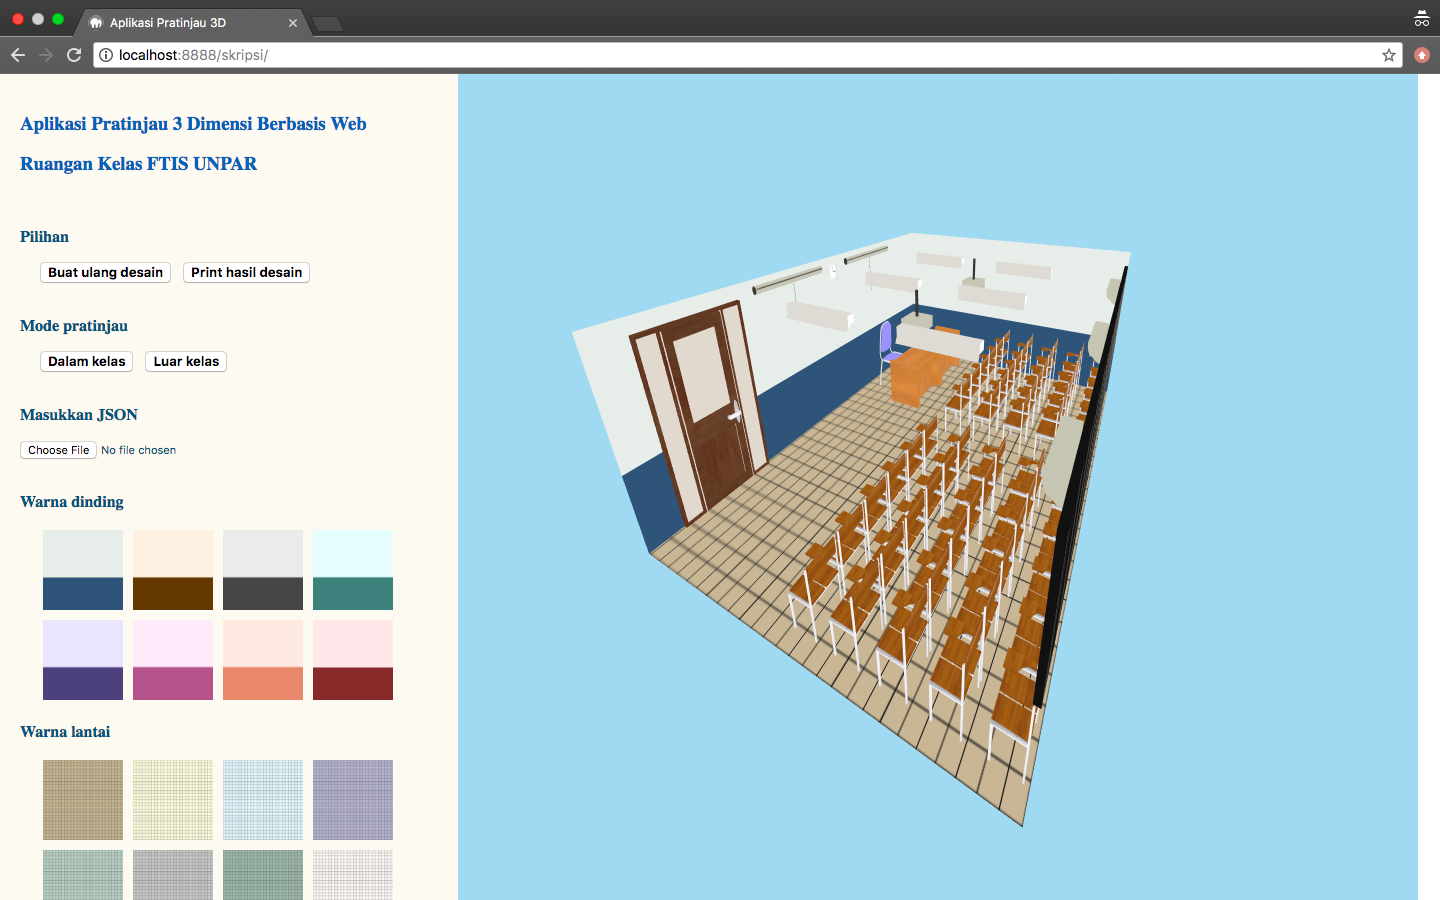
\includegraphics[scale=0.3]{tampilan}
	\caption{Tampilan akhir dari web.}
	\label{fig:tampilan}
\end{figure}

\section{Pengujian Fungsional}
\label{sec:pengujianFungsional}
Pada bagian ini akan dibahas mengenai pengujian fungsional yang dilakukan pada Aplikasi Prantijau 3 Dimensi Berbasis Web. Terdapat 15 pengujian yang dilakukan, masing-masing pengujian memiliki tujuan pengujian seperti yang dibahas pada bagian ~\ref{perancanganPengujianFungsional} dan ekspektasi yang harus dicapai oleh program.

\subsection{Mengganti Tekstur Warna Dinding Ruangan Kelas}
\label{sec:gantiteksturdinding}
Masukan untuk kasus uji ini merupakan pilihan tekstur warna dinding dari pengguna yaitu berupa warna jingga. Keluaran untuk kasus uji ini merupakan pemodelan ruangan kelas dengan warna dinding jingga sesuai dengan masukan dari pengguna. Hasil pengujian dapat dilihat pada gambar ~\ref{fig:ujidinding}.
\begin{figure}[ht]
	\centering
	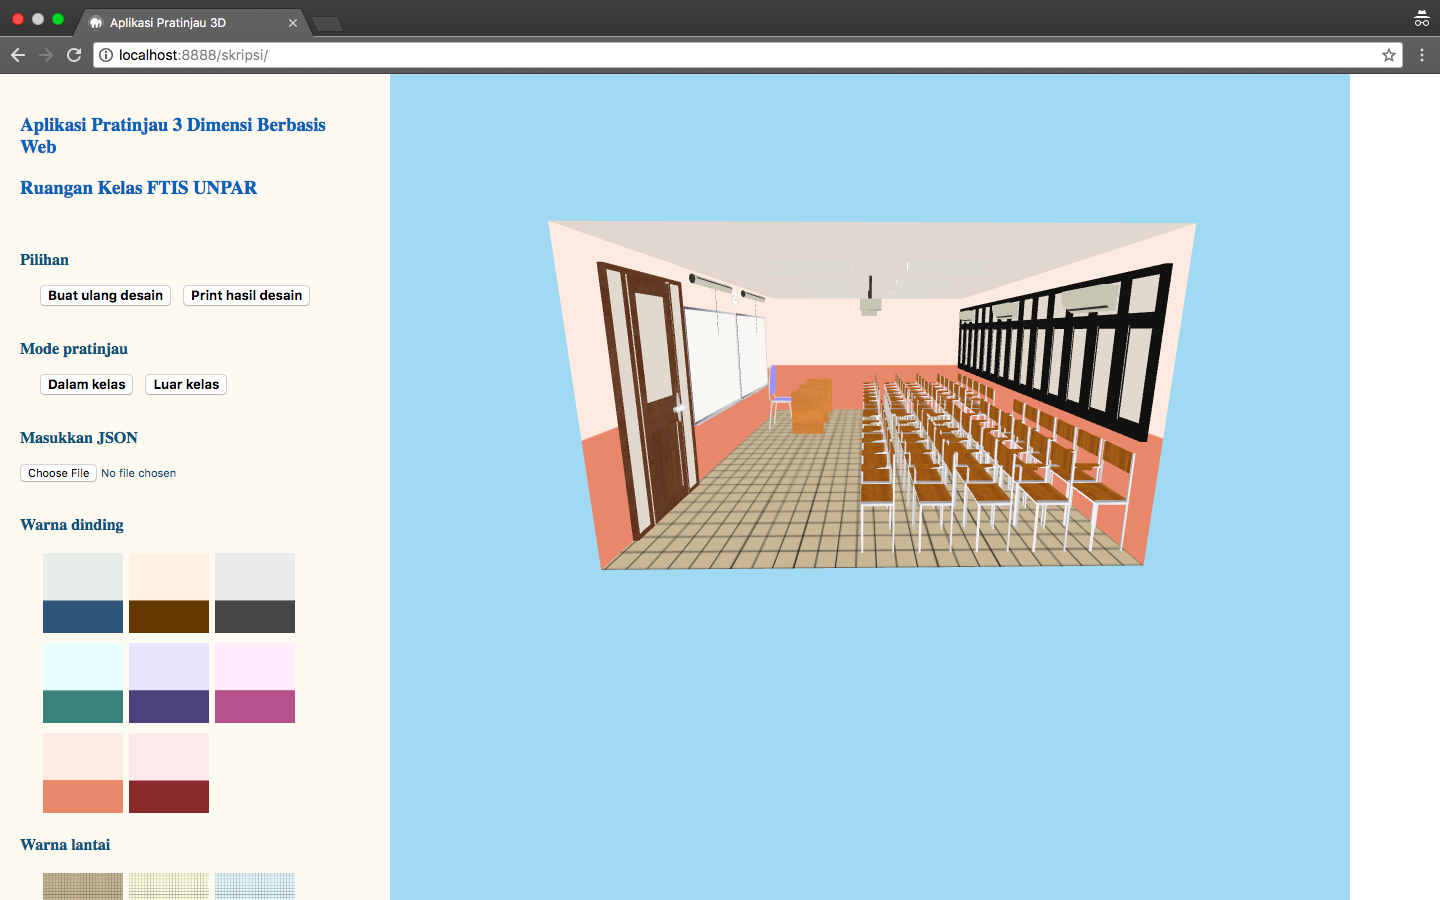
\includegraphics[scale=0.3]{ujigantidinding}
	\caption{hasil pengujian mengganti tekstur warna dinding.}
	\label{fig:ujidinding}
\end{figure}

\subsection{Mengganti Tekstur Warna Lantai Ruangan Kelas}
\label{sec:gantiteksturlantai}
Masukan untuk kasus uji ini merupakan pilihan tekstur warna lantai dari pengguna yaitu berupa warna hijau. Keluaran untuk kasus uji ini merupakan pemodelan ruangan kelas dengan warna lantai hijau sesuai dengan masukan dari pengguna. Hasil pengujian dapat dilihat pada gambar ~\ref{fig:ujilantai}.
\begin{figure}[H]
	\centering
	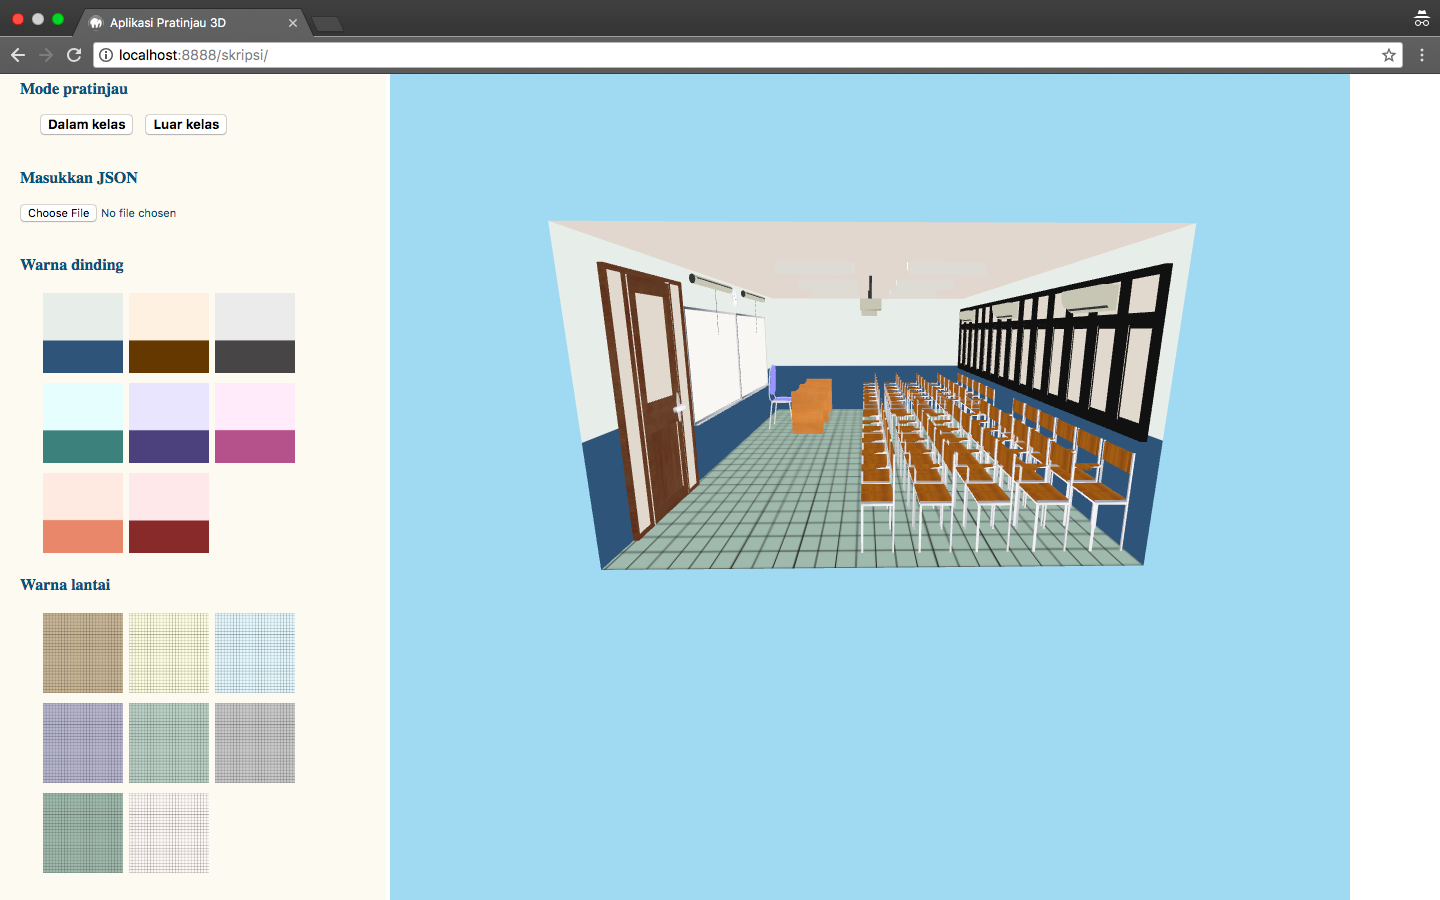
\includegraphics[scale=0.3]{ujigantilantai}
	\caption{Hasil pengujian mengganti tekstur warna lantai.}
	\label{fig:ujilantai}
\end{figure}

\subsection{Mengunggah Berkas JSON}
\label{sec:modesimulasiujian}
\begin{itemize}
	\item {\bf Ruangan kelas pada saat suasana ujian.}
	
	Masukan untuk kasus uji ini merupakan sebuah berkas JSON yang dapat dilihat pada {\it listing} ~\ref{lst:ujisuasanaujian}. Keluaran untuk kasus uji ini merupakan pemodelan ruangan kelas dengan suasana saat sedang ujian di ruangan kelas Fakultas Teknologi Informasi dan Sains. Hasil pengujian dapat dilihat pada gambar ~\ref{fig:ujisuasanaujian}.
\begin{lstlisting}[caption={Isi berkas JSON untuk pemodelan suasana ujian.}, label={lst:ujisuasanaujian},captionpos=b]
{
    "worldColor": 11131375,
    "control": {
        "minZoom": 15,
        "maxZoom": 42
    },
    "classProperties": [
        {
            "dx": 19.5,
            "dy": 4,
            "dz": 14.2,
            "distancex": -7.8,
            "distancez": -5,
            "repeatx": 6,
            "repeatz": 4,
            "rotation": 0,
            "texture": "models/texturekursimahasiswa.jpg",
            "model": "models/kursimahasiswa.json",
            "scale": 1
        },
        {
            "dx": -6,
            "dy": 10,
            "dz": -12,
            "distancex": 12.3,
            "distancez": 0,
            "repeatx": 2,
            "repeatz": 1,
            "rotation": 0,
            "texture": "models/texturepapantulis.jpg",
            "model": "models/papantulis.json",
            "scale": 3.5
        },
        {
            "dx": 19.5,
            "dy": 10.2,
            "dz": 17.1,
            "distancex": -3,
            "distancez": 0,
            "repeatx": 14,
            "repeatz": 1,
            "rotation": 3.14159,
            "texture": "models/texturejendela.jpg",
            "model": "models/jendela.json",
            "scale": 2
        },
        {
            "dx": 8,
            "dy": 4.7,
            "dz": -8,
            "distancex": 6,
            "distancez": 0,
            "repeatx": 2,
            "repeatz": 1,
            "rotation": 4.712385,
            "texture": "models/texturemejadosen.jpg",
            "model": "models/mejadosen.json",
            "scale": 2
        },
        {
            "dx": -8,
            "dy": 14.5,
            "dz": -14.9,
            "distancex": 13,
            "distancez": 0,
            "repeatx": 2,
            "repeatz": 1,
            "rotation": 0,
            "texture": "models/textureacproyektorlayar.jpg",
            "model": "models/layar.json",
            "scale": 1
        },
        {
            "dx": -4,
            "dy": 14,
            "dz": 0,
            "distancex": 13,
            "distancez": 0,
            "repeatx": 2,
            "repeatz": 1,
            "rotation": 3.14159,
            "texture": "models/textureacproyektorlayar.jpg",
            "model": "models/proyektor.json",
            "scale": 1
        },
        {
            "dx": -15,
            "dy": 13,
            "dz": 14.5,
            "distancex": 15,
            "distancez": 0,
            "repeatx": 3,
            "repeatz": 1,
            "rotation": 3.14159,
            "texture": "models/textureacproyektorlayar.jpg",
            "model": "models/ac.json",
            "scale": 1
        },
        {
            "dx": -13,
            "dy": 14.9,
            "dz": -5,
            "distancex": 10,
            "distancez": 10,
            "repeatx": 3,
            "repeatz": 2,
            "rotation": 0,
            "texture": "models/texturelampu.jpg",
            "model": "models/lampu.json",
            "scale": 1
        },
        {
            "dx": 2.7,
            "dy": 14,
            "dz": -15.2,
            "distancex": 0,
            "distancez": 0,
            "repeatx": 1,
            "repeatz": 1,
            "rotation": 0,
            "texture": "models/texturejamdinding.jpg",
            "model": "models/jamdinding.json",
            "scale": 1
        },
        {
            "dx": -13,
            "dy": 7.5,
            "dz": -14.6,
            "distancex": 0,
            "distancez": 0,
            "repeatx": 1,
            "repeatz": 1,
            "rotation": 0,
            "texture": "models/texturepintu.jpg",
            "model": "models/pintu.json",
            "scale": 2
        },
        {
            "dx": 10,
            "dy": 5.5,
            "dz": -12,
            "distancex": 0,
            "distancez": 0,
            "repeatx": 1,
            "repeatz": 1,
            "rotation": 0,
            "texture": "models/texturekursidosen.jpg",
            "model": "models/kursidosen.json",
            "scale": 1.5
        }
    ],
    "room": {
        "texture": {
            "wall": [
                "img/texturedinding1.jpg",
                "img/texturedinding2.jpg",
                "img/texturedinding3.jpg",
                "img/texturedinding4.jpg",
                "img/texturedinding5.jpg",
                "img/texturedinding6.jpg",
                "img/texturedinding7.jpg",
                "img/texturedinding8.jpg"
            ],
            "floor": [
                "img/texturelantai1.jpg",
                "img/texturelantai2.jpg",
                "img/texturelantai3.jpg",
                "img/texturelantai4.jpg",
                "img/texturelantai5.jpg",
                "img/texturelantai6.jpg",
                "img/texturelantai7.jpg",
                "img/texturelantai8.jpg"
            ],
            "ceiling": "img/textureatap.jpg"
        },
        "size": {
            "length": 43,
            "width": 12,
            "height": 31
        }
    },
    "view": {
        "outside": {
            "cameraPosition": {
                "x": 0,
                "y": 10,
                "z": 40
            },
            "control": {
                "minZoom": 10,
                "maxZoom": 42
            },
            "target": {
                "x": 0,
                "y": 10,
                "z": 0
            }
        },
        "inside": {
            "cameraPosition": {
                "x": 0,
                "y": 10,
                "z": 0
            },
            "control": {
                "minZoom": 5,
                "maxZoom": 15
            },
            "target": {
                "x": 0,
                "y": 10,
                "z": 0
            }
        },
        "init": {
            "verticalField": 75,
            "nearPlane": 0.1,
            "farPlane": 100
        }
    } 
}
\end{lstlisting}
	
\begin{figure}[H]
	\centering
	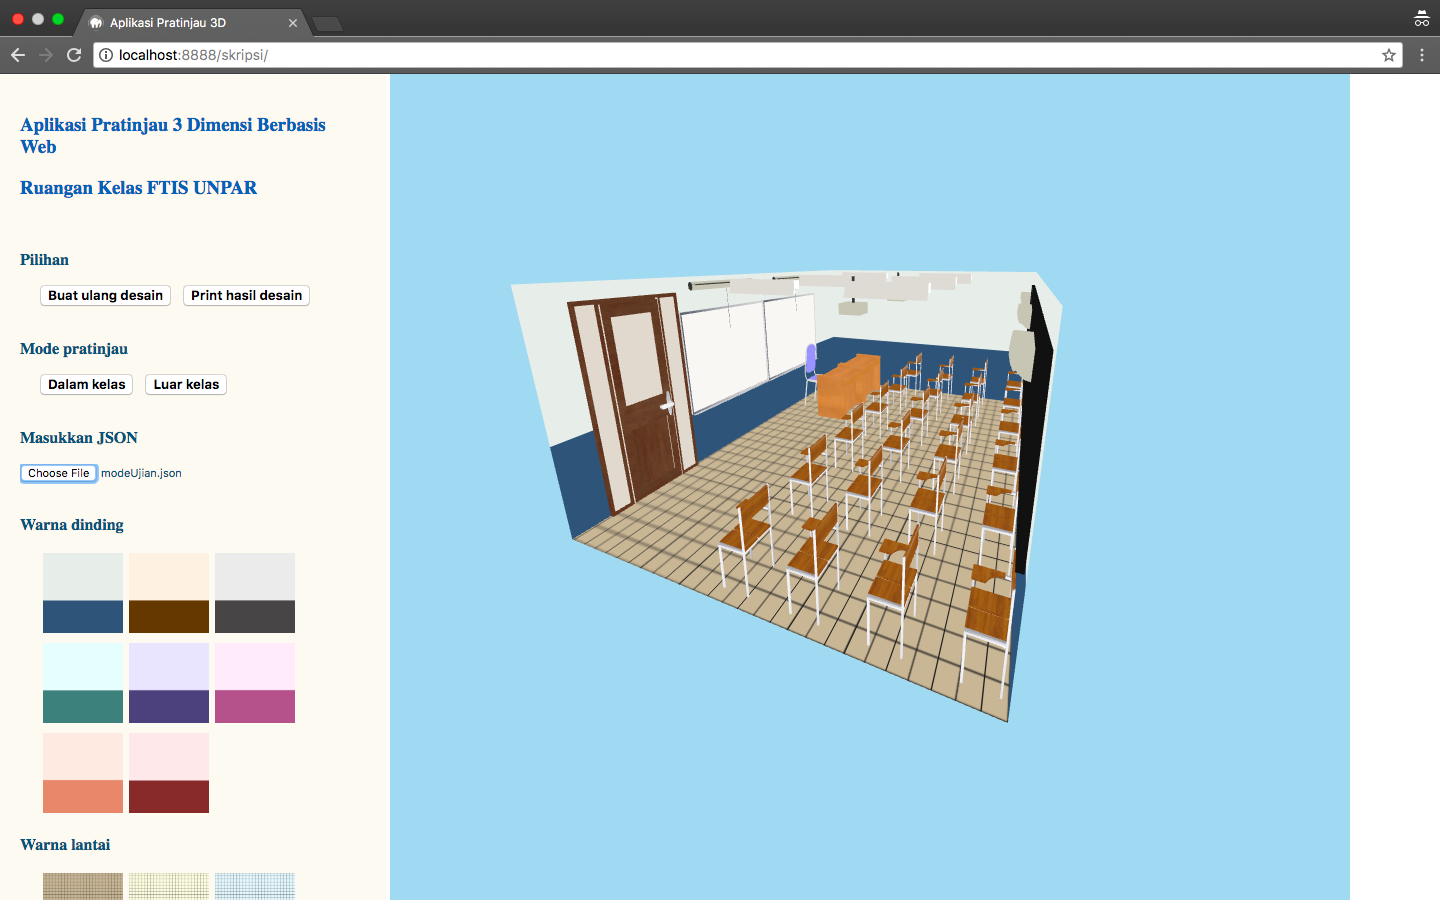
\includegraphics[scale=0.3]{ujisuasanaujian}
	\caption{Hasil pengujian pemodelan suasana ujian di ruangan kelas.}
	\label{fig:ujisuasanaujian}
\end{figure}
	
	\item {\bf Ruangan kelas pada saat tidak ada properti.}
	
	Masukan untuk kasus uji ini merupakan sebuah berkas JSON yang dapat dilihat pada {\it listing} ~\ref{lst:ujisuasanakosong}. Keluaran untuk kasus uji ini merupakan pemodelan ruangan kelas dengan suasana saat kelas kosong tanpa properti apapun di Fakultas Teknologi Informasi dan Sains. Hasil pengujian dapat dilihat pada gambar ~\ref{fig:ujisuasanakosong}.
\begin{lstlisting}[caption={Isi berkas JSON untuk pemodelan suasana kosong.}, label={lst:ujisuasanakosong},captionpos=b]
{
    "worldColor": 11131375,
    "control": {
        "minZoom": 15,
        "maxZoom": 42
    },
    "classProperties": [
        
    ],
    "room": {
        "texture": {
            "wall": [
                "img/texturedinding1.jpg",
                "img/texturedinding2.jpg",
                "img/texturedinding3.jpg",
                "img/texturedinding4.jpg",
                "img/texturedinding5.jpg",
                "img/texturedinding6.jpg",
                "img/texturedinding7.jpg",
                "img/texturedinding8.jpg"
            ],
            "floor": [
                "img/texturelantai1.jpg",
                "img/texturelantai2.jpg",
                "img/texturelantai3.jpg",
                "img/texturelantai4.jpg",
                "img/texturelantai5.jpg",
                "img/texturelantai6.jpg",
                "img/texturelantai7.jpg",
                "img/texturelantai8.jpg"
            ],
            "ceiling": "img/textureatap.jpg"
        },
        "size": {
            "length": 43,
            "width": 12,
            "height": 31
        }
    },
    "view": {
        "outside": {
            "cameraPosition": {
                "x": 0,
                "y": 10,
                "z": 40
            },
            "control": {
                "minZoom": 10,
                "maxZoom": 42
            },
            "target": {
                "x": 0,
                "y": 10,
                "z": 0
            }
        },
        "inside": {
            "cameraPosition": {
                "x": 0,
                "y": 10,
                "z": 0
            },
            "control": {
                "minZoom": 5,
                "maxZoom": 15
            },
            "target": {
                "x": 0,
                "y": 10,
                "z": 0
            }
        },
        "init": {
            "verticalField": 75,
            "nearPlane": 0.1,
            "farPlane": 100
        }
    } 
}
\end{lstlisting}

\begin{figure}[H]
	\centering
	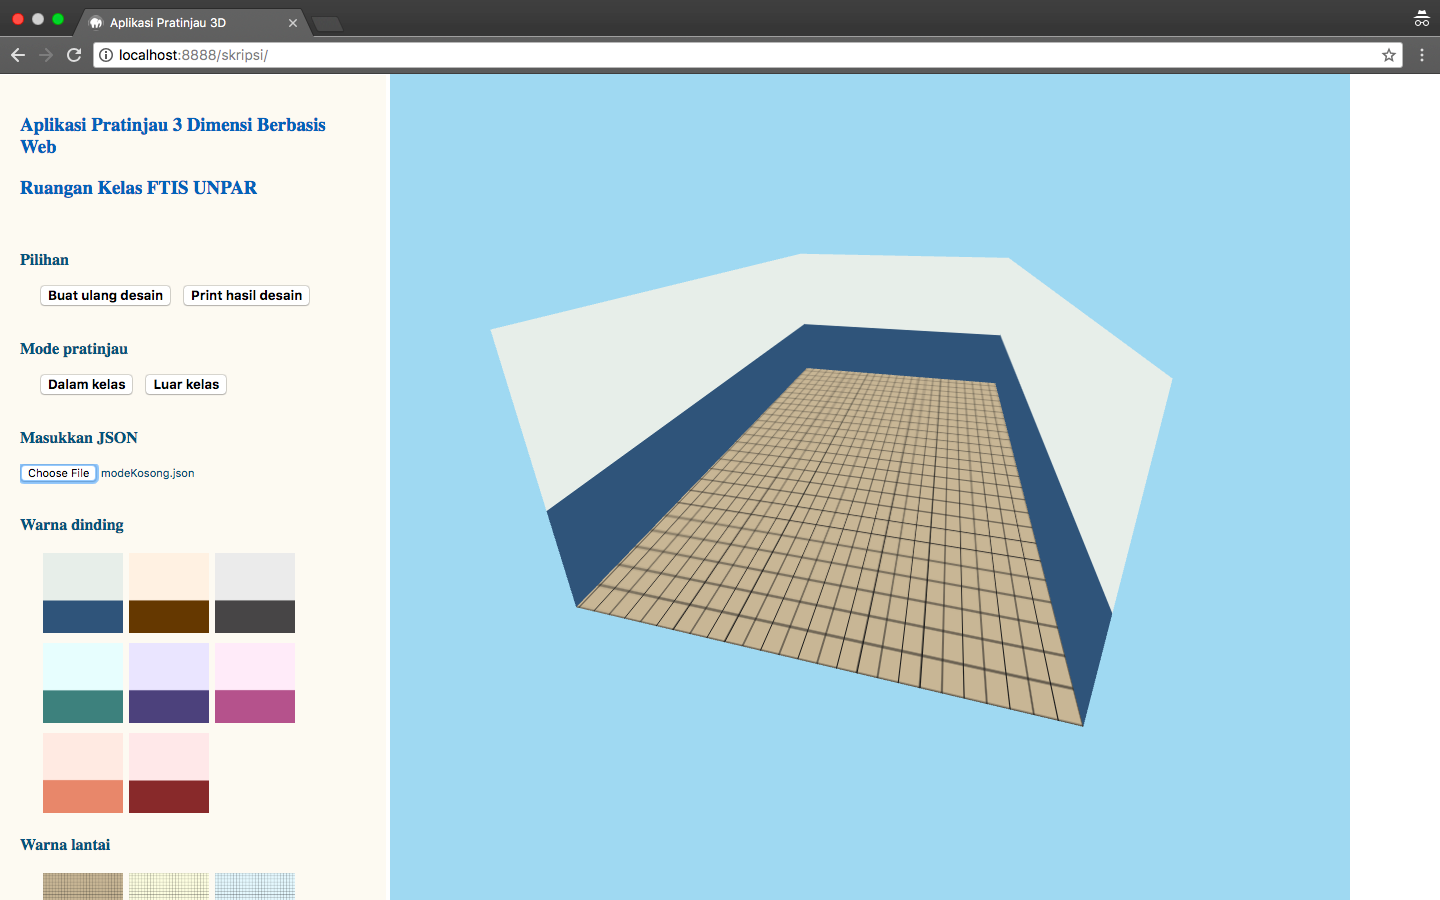
\includegraphics[scale=0.3]{ujisuasanakosong}
	\caption{Hasil pengujian pemodelan suasana saat kosong tanpa properti apapun.}
	\label{fig:ujisuasanakosong}
\end{figure}
	
	\item {\bf Ruangan kelas pada saat suasana kuliah.}
	
	Masukan untuk kasus uji ini merupakan sebuah berkas JSON yang dapat dilihat pada {\it listing} ~\ref{lst:ujisuasanakuliah}. Keluaran untuk kasus uji ini merupakan pemodelan ruangan kelas dengan suasana saat kelas sedang perkuliahan di Fakultas Teknologi Informasi dan Sains. Hasil pengujian dapat dilihat pada gambar ~\ref{fig:ujisuasanakuliah}.
\begin{lstlisting}[caption={Isi berkas JSON untuk pemodelan suasana kuliah.}, label={lst:ujisuasanakuliah},captionpos=b]
{
    "worldColor": 11131375,
    "control": {
        "minZoom": 15,
        "maxZoom": 42
    },
    "classProperties": [
        {
            "dx": 19.5,
            "dy": 4,
            "dz": 14.2,
            "distancex": -3,
            "distancez": -3.5,
            "repeatx": 6,
            "repeatz": 5,
            "rotation": 0,
            "texture": "models/texturekursimahasiswa.jpg",
            "model": "models/kursimahasiswa.json",
            "scale": 1
        },
        {
            "dx": -4,
            "dy": 4,
            "dz": 14.2,
            "distancex": -3,
            "distancez": -3.5,
            "repeatx": 6,
            "repeatz": 5,
            "rotation": 0,
            "texture": "models/texturekursimahasiswa.jpg",
            "model": "models/kursimahasiswa.json",
            "scale": 1
        },
        {
            "dx": -6,
            "dy": 10,
            "dz": -12,
            "distancex": 12.3,
            "distancez": 0,
            "repeatx": 2,
            "repeatz": 1,
            "rotation": 0,
            "texture": "models/texturepapantulis.jpg",
            "model": "models/papantulis.json",
            "scale": 3.5
        },
        {
            "dx": 19.5,
            "dy": 10.2,
            "dz": 17.1,
            "distancex": -3,
            "distancez": 0,
            "repeatx": 14,
            "repeatz": 1,
            "rotation": 3.14159,
            "texture": "models/texturejendela.jpg",
            "model": "models/jendela.json",
            "scale": 2
        },
        {
            "dx": 8,
            "dy": 4.7,
            "dz": -8,
            "distancex": 6,
            "distancez": 0,
            "repeatx": 2,
            "repeatz": 1,
            "rotation": 4.712385,
            "texture": "models/texturemejadosen.jpg",
            "model": "models/mejadosen.json",
            "scale": 2
        },
        {
            "dx": -8,
            "dy": 14.5,
            "dz": -14.9,
            "distancex": 13,
            "distancez": 0,
            "repeatx": 2,
            "repeatz": 1,
            "rotation": 0,
            "texture": "models/textureacproyektorlayar.jpg",
            "model": "models/layar.json",
            "scale": 1
        },
        {
            "dx": -4,
            "dy": 14,
            "dz": 0,
            "distancex": 13,
            "distancez": 0,
            "repeatx": 2,
            "repeatz": 1,
            "rotation": 3.14159,
            "texture": "models/textureacproyektorlayar.jpg",
            "model": "models/proyektor.json",
            "scale": 1
        },
        {
            "dx": -15,
            "dy": 13,
            "dz": 14.5,
            "distancex": 15,
            "distancez": 0,
            "repeatx": 3,
            "repeatz": 1,
            "rotation": 3.14159,
            "texture": "models/textureacproyektorlayar.jpg",
            "model": "models/ac.json",
            "scale": 1
        },
        {
            "dx": -13,
            "dy": 14.9,
            "dz": -5,
            "distancex": 10,
            "distancez": 10,
            "repeatx": 3,
            "repeatz": 2,
            "rotation": 0,
            "texture": "models/texturelampu.jpg",
            "model": "models/lampu.json",
            "scale": 1
        },
        {
            "dx": 2.7,
            "dy": 14,
            "dz": -15.2,
            "distancex": 0,
            "distancez": 0,
            "repeatx": 1,
            "repeatz": 1,
            "rotation": 0,
            "texture": "models/texturejamdinding.jpg",
            "model": "models/jamdinding.json",
            "scale": 1
        },
        {
            "dx": -13,
            "dy": 7.5,
            "dz": -14.6,
            "distancex": 0,
            "distancez": 0,
            "repeatx": 1,
            "repeatz": 1,
            "rotation": 0,
            "texture": "models/texturepintu.jpg",
            "model": "models/pintu.json",
            "scale": 2
        },
        {
            "dx": 10,
            "dy": 5.5,
            "dz": -12,
            "distancex": 0,
            "distancez": 0,
            "repeatx": 1,
            "repeatz": 1,
            "rotation": 0,
            "texture": "models/texturekursidosen.jpg",
            "model": "models/kursidosen.json",
            "scale": 1.5
        }
    ],
    "room": {
        "texture": {
            "wall": [
                "img/texturedinding1.jpg",
                "img/texturedinding2.jpg",
                "img/texturedinding3.jpg",
                "img/texturedinding4.jpg",
                "img/texturedinding5.jpg",
                "img/texturedinding6.jpg",
                "img/texturedinding7.jpg",
                "img/texturedinding8.jpg"
            ],
            "floor": [
                "img/texturelantai1.jpg",
                "img/texturelantai2.jpg",
                "img/texturelantai3.jpg",
                "img/texturelantai4.jpg",
                "img/texturelantai5.jpg",
                "img/texturelantai6.jpg",
                "img/texturelantai7.jpg",
                "img/texturelantai8.jpg"
            ],
            "ceiling": "img/textureatap.jpg"
        },
        "size": {
            "length": 43,
            "width": 12,
            "height": 31
        }
    },
    "view": {
        "outside": {
            "cameraPosition": {
                "x": 0,
                "y": 10,
                "z": 40
            },
            "control": {
                "minZoom": 10,
                "maxZoom": 42
            },
            "target": {
                "x": 0,
                "y": 10,
                "z": 0
            }
        },
        "inside": {
            "cameraPosition": {
                "x": 0,
                "y": 10,
                "z": 0
            },
            "control": {
                "minZoom": 5,
                "maxZoom": 15
            },
            "target": {
                "x": 0,
                "y": 10,
                "z": 0
            }
        },
        "init": {
            "verticalField": 75,
            "nearPlane": 0.1,
            "farPlane": 100
        }
    } 
}
\end{lstlisting}

\begin{figure}[H]
	\centering
	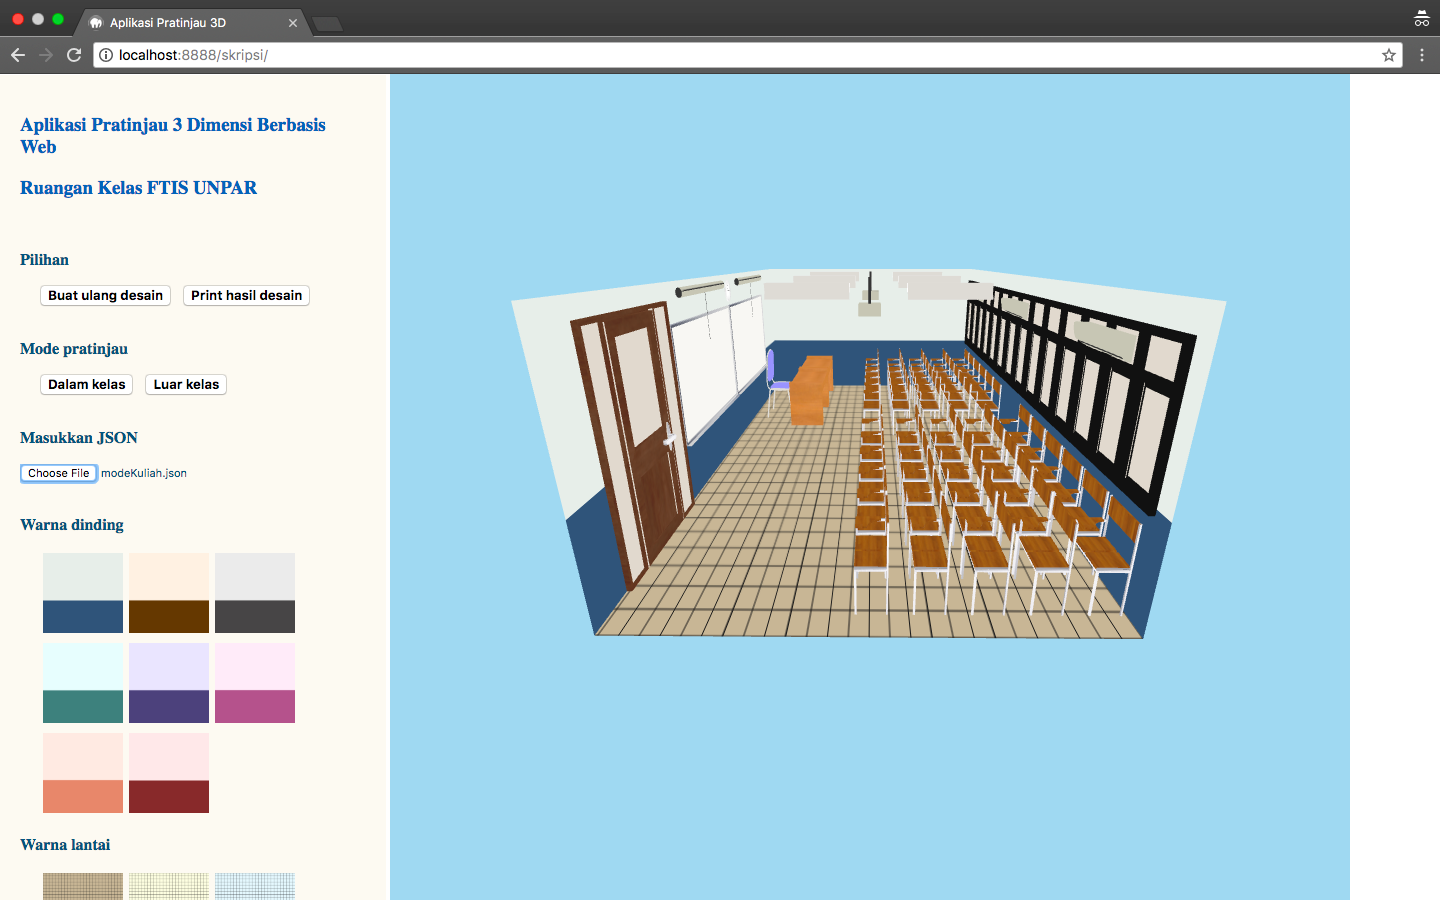
\includegraphics[scale=0.3]{ujisuasanakuliah}
	\caption{Hasil pengujian pemodelan suasana saat kuliah di ruangan kelas.}
	\label{fig:ujisuasanakuliah}
\end{figure}
	
	\item {\bf Ruangan kelas pada saat tidak ada pendingin ruangan.}
	
	Masukan untuk kasus uji ini merupakan sebuah berkas JSON yang dapat dilihat pada {\it listing} ~\ref{lst:ujitanpaac}. Keluaran untuk kasus uji ini merupakan pemodelan ruangan kelas tanpa pendingin ruangan. Hasil pengujian dapat dilihat pada gambar ~\ref{fig:ujitanpaac}.
\begin{lstlisting}[caption={Isi berkas JSON untuk pemodelan ruangan kelas tanpa pendingin.}, label={lst:ujitanpaac},captionpos=b]
{
    "worldColor": 11131375,
    "control": {
        "minZoom": 15,
        "maxZoom": 42
    },
    "classProperties": [
        {
            "dx": 19.5,
            "dy": 4,
            "dz": 14.2,
            "distancex": -3,
            "distancez": -3.5,
            "repeatx": 6,
            "repeatz": 5,
            "rotation": 0,
            "texture": "models/texturekursimahasiswa.jpg",
            "model": "models/kursimahasiswa.json",
            "scale": 1
        },
        {
            "dx": -4,
            "dy": 4,
            "dz": 14.2,
            "distancex": -3,
            "distancez": -3.5,
            "repeatx": 6,
            "repeatz": 5,
            "rotation": 0,
            "texture": "models/texturekursimahasiswa.jpg",
            "model": "models/kursimahasiswa.json",
            "scale": 1
        },
        {
            "dx": -6,
            "dy": 10,
            "dz": -12,
            "distancex": 12.3,
            "distancez": 0,
            "repeatx": 2,
            "repeatz": 1,
            "rotation": 0,
            "texture": "models/texturepapantulis.jpg",
            "model": "models/papantulis.json",
            "scale": 3.5
        },
        {
            "dx": 19.5,
            "dy": 10.2,
            "dz": 17.1,
            "distancex": -3,
            "distancez": 0,
            "repeatx": 14,
            "repeatz": 1,
            "rotation": 3.14159,
            "texture": "models/texturejendela.jpg",
            "model": "models/jendela.json",
            "scale": 2
        },
        {
            "dx": 8,
            "dy": 4.7,
            "dz": -8,
            "distancex": 6,
            "distancez": 0,
            "repeatx": 2,
            "repeatz": 1,
            "rotation": 4.712385,
            "texture": "models/texturemejadosen.jpg",
            "model": "models/mejadosen.json",
            "scale": 2
        },
        {
            "dx": -8,
            "dy": 14.5,
            "dz": -14.9,
            "distancex": 13,
            "distancez": 0,
            "repeatx": 2,
            "repeatz": 1,
            "rotation": 0,
            "texture": "models/textureacproyektorlayar.jpg",
            "model": "models/layar.json",
            "scale": 1
        },
        {
            "dx": -4,
            "dy": 14,
            "dz": 0,
            "distancex": 13,
            "distancez": 0,
            "repeatx": 2,
            "repeatz": 1,
            "rotation": 3.14159,
            "texture": "models/textureacproyektorlayar.jpg",
            "model": "models/proyektor.json",
            "scale": 1
        },
        {
            "dx": -13,
            "dy": 14.9,
            "dz": -5,
            "distancex": 10,
            "distancez": 10,
            "repeatx": 3,
            "repeatz": 2,
            "rotation": 0,
            "texture": "models/texturelampu.jpg",
            "model": "models/lampu.json",
            "scale": 1
        },
        {
            "dx": 2.7,
            "dy": 14,
            "dz": -15.2,
            "distancex": 0,
            "distancez": 0,
            "repeatx": 1,
            "repeatz": 1,
            "rotation": 0,
            "texture": "models/texturejamdinding.jpg",
            "model": "models/jamdinding.json",
            "scale": 1
        },
        {
            "dx": -13,
            "dy": 7.5,
            "dz": -14.6,
            "distancex": 0,
            "distancez": 0,
            "repeatx": 1,
            "repeatz": 1,
            "rotation": 0,
            "texture": "models/texturepintu.jpg",
            "model": "models/pintu.json",
            "scale": 2
        },
        {
            "dx": 10,
            "dy": 5.5,
            "dz": -12,
            "distancex": 0,
            "distancez": 0,
            "repeatx": 1,
            "repeatz": 1,
            "rotation": 0,
            "texture": "models/texturekursidosen.jpg",
            "model": "models/kursidosen.json",
            "scale": 1.5
        }
    ],
    "room": {
        "texture": {
            "wall": [
                "img/texturedinding1.jpg",
                "img/texturedinding2.jpg",
                "img/texturedinding3.jpg",
                "img/texturedinding4.jpg",
                "img/texturedinding5.jpg",
                "img/texturedinding6.jpg",
                "img/texturedinding7.jpg",
                "img/texturedinding8.jpg"
            ],
            "floor": [
                "img/texturelantai1.jpg",
                "img/texturelantai2.jpg",
                "img/texturelantai3.jpg",
                "img/texturelantai4.jpg",
                "img/texturelantai5.jpg",
                "img/texturelantai6.jpg",
                "img/texturelantai7.jpg",
                "img/texturelantai8.jpg"
            ],
            "ceiling": "img/textureatap.jpg"
        },
        "size": {
            "length": 43,
            "width": 12,
            "height": 31
        }
    },
    "view": {
        "outside": {
            "cameraPosition": {
                "x": 0,
                "y": 10,
                "z": 40
            },
            "control": {
                "minZoom": 10,
                "maxZoom": 42
            },
            "target": {
                "x": 0,
                "y": 10,
                "z": 0
            }
        },
        "inside": {
            "cameraPosition": {
                "x": 0,
                "y": 10,
                "z": 0
            },
            "control": {
                "minZoom": 5,
                "maxZoom": 15
            },
            "target": {
                "x": 0,
                "y": 10,
                "z": 0
            }
        },
        "init": {
            "verticalField": 75,
            "nearPlane": 0.1,
            "farPlane": 100
        }
    } 
}
\end{lstlisting}

\begin{figure}[H]
	\centering
	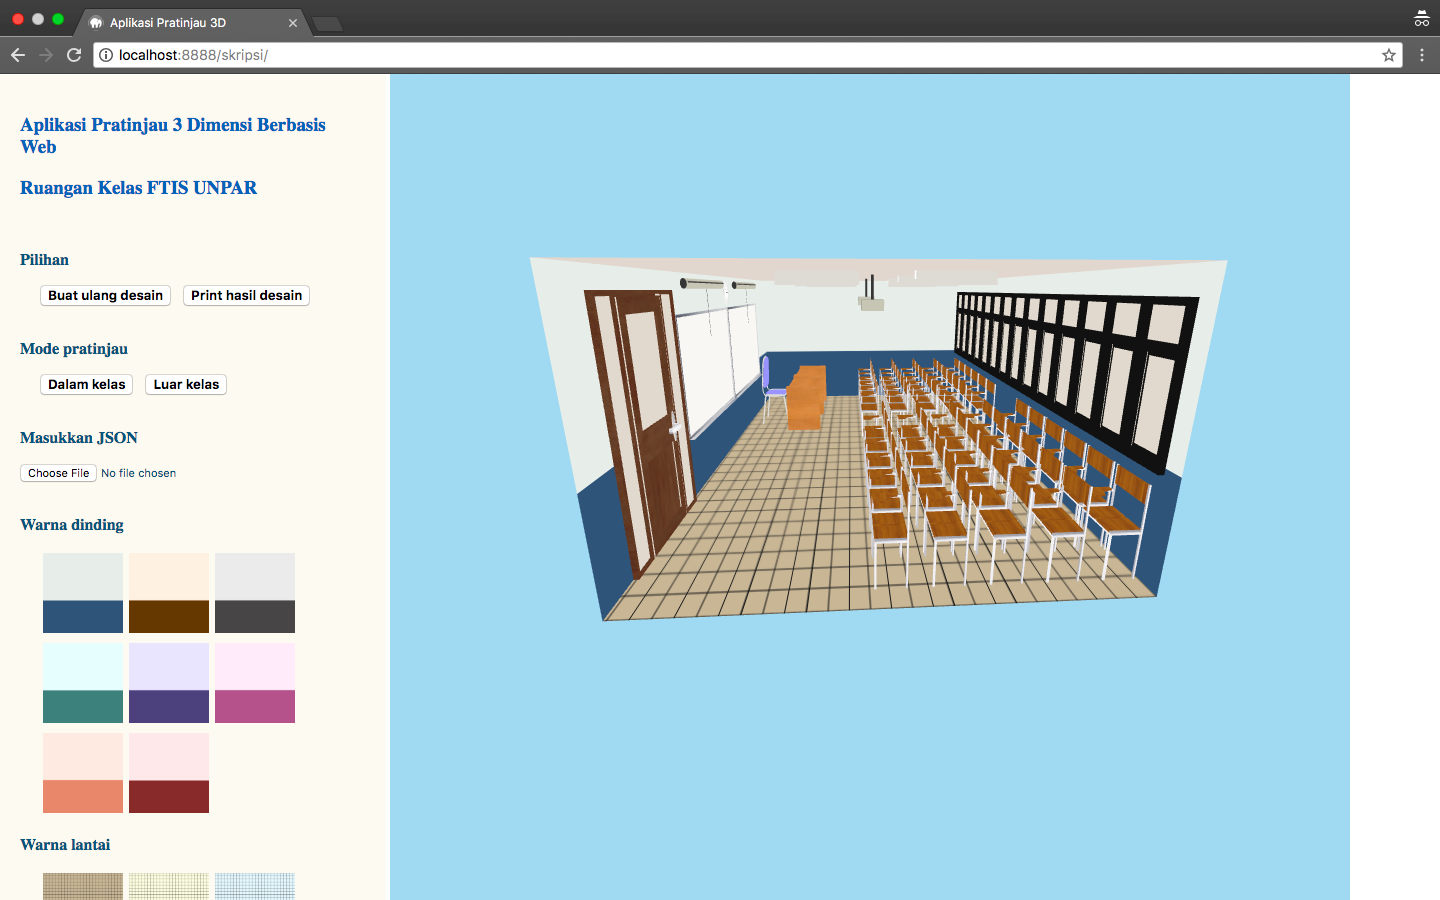
\includegraphics[scale=0.3]{ujitanpaac}
	\caption{Hasil pengujian pemodelan ruangan kelas tanpa pendingin.}
	\label{fig:ujitanpaac}
\end{figure}
	
	\item {\bf Ruangan kelas pada saat hanya ada satu kursi di tengah ruangan.}
	
	Masukan untuk kasus uji ini merupakan sebuah berkas JSON yang dapat dilihat pada {\it listing} ~\ref{lst:ujisatukursi}. Keluaran untuk kasus uji ini merupakan pemodelan ruangan kelas dengan hanya satu properti kursi mahasiswa di dalamnya. Hasil pengujian dapat dilihat pada gambar ~\ref{fig:ujisatukursi}.
\begin{lstlisting}[caption={Isi berkas JSON untuk pemodelan ruangan kelas hanya dengan satu kursi.}, label={lst:ujisatukursi},captionpos=b]
{
        "worldColor": 11131375,
        "control": {
            "minZoom": 15,
            "maxZoom": 42
        },
        "classProperties": [
        {
            "dx": 0.5,
            "dy": 4,
            "dz": -1.2,
            "distancex": -3,
            "distancez": -3.5,
            "repeatx": 1,
            "repeatz": 1,
            "rotation": 0,
            "texture": "models/texturekursimahasiswa.jpg",
            "model": "models/kursimahasiswa.json",
            "scale": 1
        }
    ],
    "room": {
        "texture": {
            "wall": [
                "img/texturedinding1.jpg",
                "img/texturedinding2.jpg",
                "img/texturedinding3.jpg",
                "img/texturedinding4.jpg",
                "img/texturedinding5.jpg",
                "img/texturedinding6.jpg",
                "img/texturedinding7.jpg",
                "img/texturedinding8.jpg"
            ],
            "floor": [
                "img/texturelantai1.jpg",
                "img/texturelantai2.jpg",
                "img/texturelantai3.jpg",
                "img/texturelantai4.jpg",
                "img/texturelantai5.jpg",
                "img/texturelantai6.jpg",
                "img/texturelantai7.jpg",
                "img/texturelantai8.jpg"
            ],
            "ceiling": "img/textureatap.jpg"
        },
        "size": {
            "length": 43,
            "width": 12,
            "height": 31
        }
    },
    "view": {
        "outside": {
            "cameraPosition": {
                "x": 0,
                "y": 10,
                "z": 40
            },
            "control": {
                "minZoom": 10,
                "maxZoom": 42
            },
            "target": {
                "x": 0,
                "y": 10,
                "z": 0
            }
        },
        "inside": {
            "cameraPosition": {
                "x": 0,
                "y": 10,
                "z": 0
            },
            "control": {
                "minZoom": 5,
                "maxZoom": 15
            },
            "target": {
                "x": 0,
                "y": 10,
                "z": 0
            }
        },
        "init": {
            "verticalField": 75,
            "nearPlane": 0.1,
            "farPlane": 100
        }
    } 
}
\end{lstlisting}

\begin{figure}[H]
	\centering
	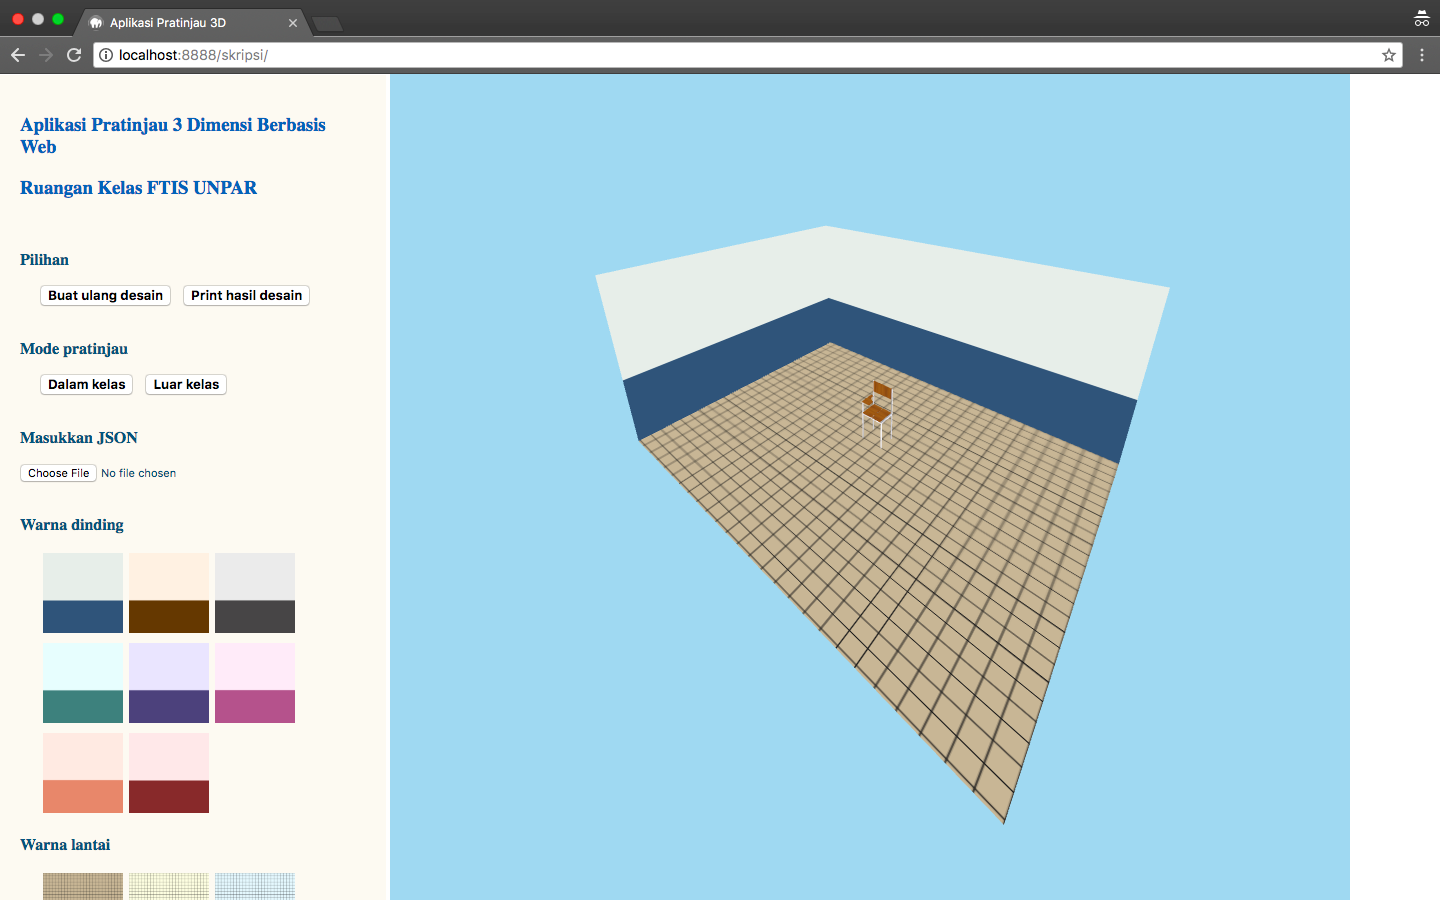
\includegraphics[scale=0.3]{ujisatukursi}
	\caption{Hasil pengujian pemodelan ruangan kelas hanya dengan satu kursi.}
	\label{fig:ujisatukursi}
\end{figure}
	
	\item {\bf Ruangan kelas pada saat suasana ujian dengan dua meja pengawas.}
	
	Masukan untuk kasus uji ini merupakan sebuah berkas JSON yang dapat dilihat pada {\it listing} ~\ref{lst:ujiduamejadosen}. Keluaran untuk kasus uji ini merupakan pemodelan ruangan kelas dengan dua properti meja dosen pada saat suasana ujian. Hasil pengujian dapat dilihat pada gambar ~\ref{fig:ujiduamejadosen}.
\begin{lstlisting}[caption={Isi berkas JSON untuk pemodelan ruangan kelas dengan dua meja dosen.}, label={lst:ujiduamejadosen},captionpos=b]
{
    "worldColor": 11131375,
    "control": {
        "minZoom": 15,
        "maxZoom": 42
    },
    "classProperties": [
        {
            "dx": 19.5,
            "dy": 4,
            "dz": 14.2,
            "distancex": -7.8,
            "distancez": -5,
            "repeatx": 6,
            "repeatz": 4,
            "rotation": 0,
            "texture": "models/texturekursimahasiswa.jpg",
            "model": "models/kursimahasiswa.json",
            "scale": 1
        },
        {
            "dx": -6,
            "dy": 10,
            "dz": -12,
            "distancex": 12.3,
            "distancez": 0,
            "repeatx": 2,
            "repeatz": 1,
            "rotation": 0,
            "texture": "models/texturepapantulis.jpg",
            "model": "models/papantulis.json",
            "scale": 3.5
        },
        {
            "dx": 19.5,
            "dy": 10.2,
            "dz": 17.1,
            "distancex": -3,
            "distancez": 0,
            "repeatx": 14,
            "repeatz": 1,
            "rotation": 3.14159,
            "texture": "models/texturejendela.jpg",
            "model": "models/jendela.json",
            "scale": 2
        },
        {
            "dx": -2,
            "dy": 4.7,
            "dz": -8,
            "distancex": 15,
            "distancez": 0,
            "repeatx": 2,
            "repeatz": 1,
            "rotation": 4.712385,
            "texture": "models/texturemejadosen.jpg",
            "model": "models/mejadosen.json",
            "scale": 2
        },
        {
            "dx": -8,
            "dy": 14.5,
            "dz": -14.9,
            "distancex": 13,
            "distancez": 0,
            "repeatx": 2,
            "repeatz": 1,
            "rotation": 0,
            "texture": "models/textureacproyektorlayar.jpg",
            "model": "models/layar.json",
            "scale": 1
        },
        {
            "dx": -4,
            "dy": 14,
            "dz": 0,
            "distancex": 13,
            "distancez": 0,
            "repeatx": 2,
            "repeatz": 1,
            "rotation": 3.14159,
            "texture": "models/textureacproyektorlayar.jpg",
            "model": "models/proyektor.json",
            "scale": 1
        },
        {
            "dx": -15,
            "dy": 13,
            "dz": 14.5,
            "distancex": 15,
            "distancez": 0,
            "repeatx": 3,
            "repeatz": 1,
            "rotation": 3.14159,
            "texture": "models/textureacproyektorlayar.jpg",
            "model": "models/ac.json",
            "scale": 1
        },
        {
            "dx": -13,
            "dy": 14.9,
            "dz": -5,
            "distancex": 10,
            "distancez": 10,
            "repeatx": 3,
            "repeatz": 2,
            "rotation": 0,
            "texture": "models/texturelampu.jpg",
            "model": "models/lampu.json",
            "scale": 1
        },
        {
            "dx": 2.7,
            "dy": 14,
            "dz": -15.2,
            "distancex": 0,
            "distancez": 0,
            "repeatx": 1,
            "repeatz": 1,
            "rotation": 0,
            "texture": "models/texturejamdinding.jpg",
            "model": "models/jamdinding.json",
            "scale": 1
        },
        {
            "dx": -13,
            "dy": 7.5,
            "dz": -14.6,
            "distancex": 0,
            "distancez": 0,
            "repeatx": 1,
            "repeatz": 1,
            "rotation": 0,
            "texture": "models/texturepintu.jpg",
            "model": "models/pintu.json",
            "scale": 2
        },
        {
            "dx": 0,
            "dy": 5.5,
            "dz": -12,
            "distancex": 15,
            "distancez": 0,
            "repeatx": 2,
            "repeatz": 1,
            "rotation": 0,
            "texture": "models/texturekursidosen.jpg",
            "model": "models/kursidosen.json",
            "scale": 1.5
        }
    ],
    "room": {
        "texture": {
            "wall": [
                "img/texturedinding1.jpg",
                "img/texturedinding2.jpg",
                "img/texturedinding3.jpg",
                "img/texturedinding4.jpg",
                "img/texturedinding5.jpg",
                "img/texturedinding6.jpg",
                "img/texturedinding7.jpg",
                "img/texturedinding8.jpg"
            ],
            "floor": [
                "img/texturelantai1.jpg",
                "img/texturelantai2.jpg",
                "img/texturelantai3.jpg",
                "img/texturelantai4.jpg",
                "img/texturelantai5.jpg",
                "img/texturelantai6.jpg",
                "img/texturelantai7.jpg",
                "img/texturelantai8.jpg"
            ],
            "ceiling": "img/textureatap.jpg"
        },
        "size": {
            "length": 43,
            "width": 12,
            "height": 31
        }
    },
    "view": {
        "outside": {
            "cameraPosition": {
                "x": 0,
                "y": 10,
                "z": 40
            },
            "control": {
                "minZoom": 10,
                "maxZoom": 42
            },
            "target": {
                "x": 0,
                "y": 10,
                "z": 0
            }
        },
        "inside": {
            "cameraPosition": {
                "x": 0,
                "y": 10,
                "z": 0
            },
            "control": {
                "minZoom": 5,
                "maxZoom": 15
            },
            "target": {
                "x": 0,
                "y": 10,
                "z": 0
            }
        },
        "init": {
            "verticalField": 75,
            "nearPlane": 0.1,
            "farPlane": 100
        }
    } 
}
\end{lstlisting}

\begin{figure}[H]
	\centering
	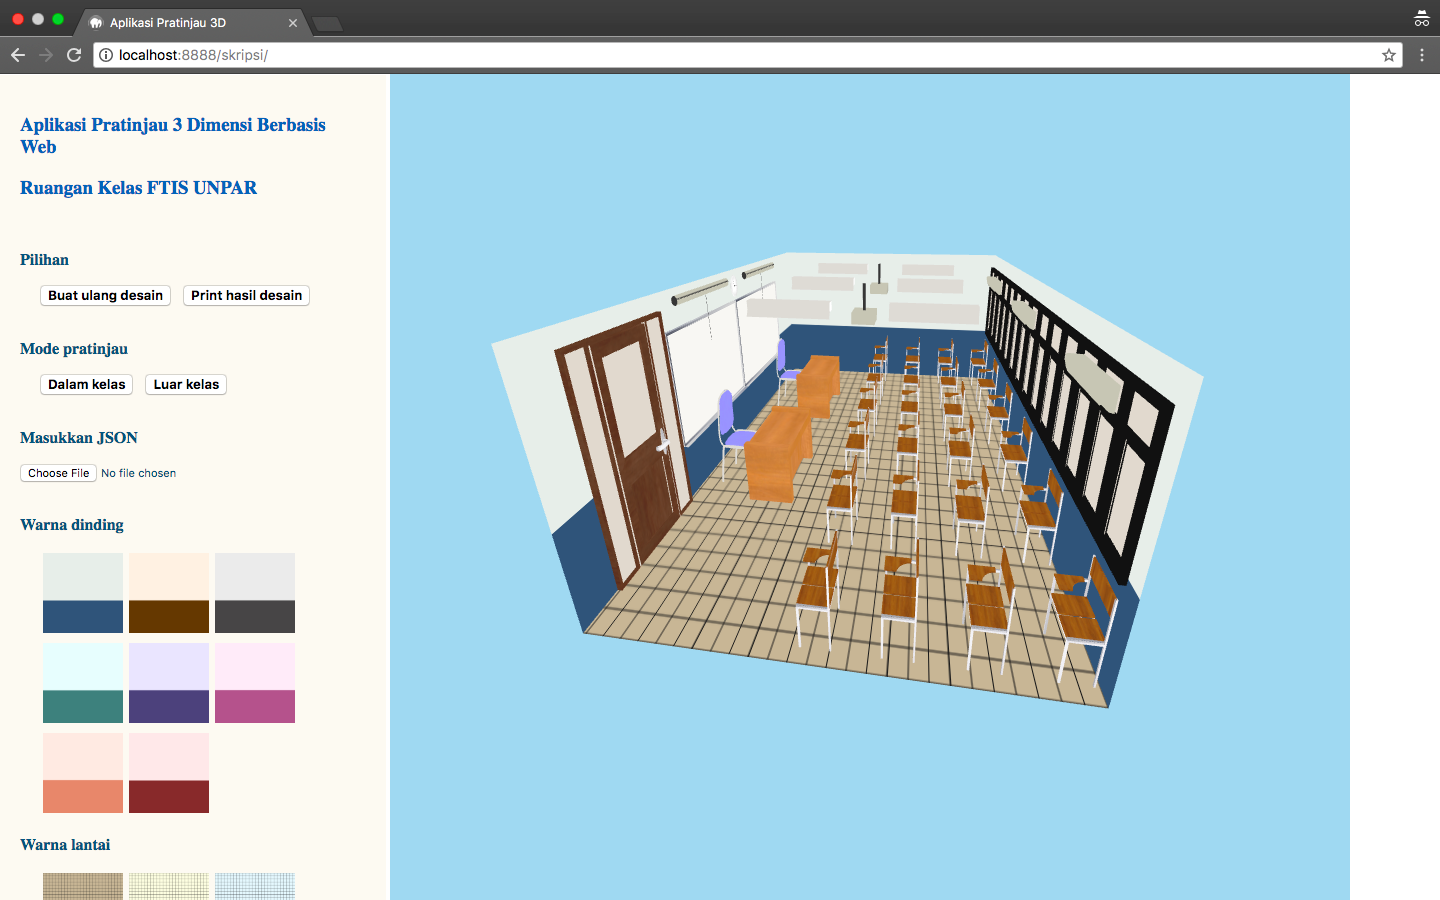
\includegraphics[scale=0.3]{ujiduamejadosen}
	\caption{Hasil pengujian pemodelan ruangan kelas dengan dua meja dosen}
	\label{fig:ujiduamejadosen}
\end{figure}
	
	\item {\bf Ruangan kelas pada saat suasana ujian tanpa ada meja pengawas.}
	
	Masukan untuk kasus uji ini merupakan sebuah berkas JSON yang dapat dilihat pada {\it listing} ~\ref{lst:ujitanpamejadosen}. Keluaran untuk kasus uji ini merupakan pemodelan ruangan kelas tanpa properti meja dosen pada saat suasana ujian. Hasil pengujian dapat dilihat pada gambar ~\ref{fig:ujitanpamejadosen}.
\begin{lstlisting}[caption={Isi berkas JSON untuk pemodelan ruangan kelas tanpa meja dosen.}, label={lst:ujitanpamejadosen},captionpos=b]
{
    "worldColor": 11131375,
    "control": {
        "minZoom": 15,
        "maxZoom": 42
    },
    "classProperties": [
        {
            "dx": 19.5,
            "dy": 4,
            "dz": 14.2,
            "distancex": -7.8,
            "distancez": -5,
            "repeatx": 6,
            "repeatz": 4,
            "rotation": 0,
            "texture": "models/texturekursimahasiswa.jpg",
            "model": "models/kursimahasiswa.json",
            "scale": 1
        },
        {
            "dx": -6,
            "dy": 10,
            "dz": -12,
            "distancex": 12.3,
            "distancez": 0,
            "repeatx": 2,
            "repeatz": 1,
            "rotation": 0,
            "texture": "models/texturepapantulis.jpg",
            "model": "models/papantulis.json",
            "scale": 3.5
        },
        {
            "dx": 19.5,
            "dy": 10.2,
            "dz": 17.1,
            "distancex": -3,
            "distancez": 0,
            "repeatx": 14,
            "repeatz": 1,
            "rotation": 3.14159,
            "texture": "models/texturejendela.jpg",
            "model": "models/jendela.json",
            "scale": 2
        },
        {
            "dx": -8,
            "dy": 14.5,
            "dz": -14.9,
            "distancex": 13,
            "distancez": 0,
            "repeatx": 2,
            "repeatz": 1,
            "rotation": 0,
            "texture": "models/textureacproyektorlayar.jpg",
            "model": "models/layar.json",
            "scale": 1
        },
        {
            "dx": -4,
            "dy": 14,
            "dz": 0,
            "distancex": 13,
            "distancez": 0,
            "repeatx": 2,
            "repeatz": 1,
            "rotation": 3.14159,
            "texture": "models/textureacproyektorlayar.jpg",
            "model": "models/proyektor.json",
            "scale": 1
        },
        {
            "dx": -15,
            "dy": 13,
            "dz": 14.5,
            "distancex": 15,
            "distancez": 0,
            "repeatx": 3,
            "repeatz": 1,
            "rotation": 3.14159,
            "texture": "models/textureacproyektorlayar.jpg",
            "model": "models/ac.json",
            "scale": 1
        },
        {
            "dx": -13,
            "dy": 14.9,
            "dz": -5,
            "distancex": 10,
            "distancez": 10,
            "repeatx": 3,
            "repeatz": 2,
            "rotation": 0,
            "texture": "models/texturelampu.jpg",
            "model": "models/lampu.json",
            "scale": 1
        },
        {
            "dx": 2.7,
            "dy": 14,
            "dz": -15.2,
            "distancex": 0,
            "distancez": 0,
            "repeatx": 1,
            "repeatz": 1,
            "rotation": 0,
            "texture": "models/texturejamdinding.jpg",
            "model": "models/jamdinding.json",
            "scale": 1
        },
        {
            "dx": -13,
            "dy": 7.5,
            "dz": -14.6,
            "distancex": 0,
            "distancez": 0,
            "repeatx": 1,
            "repeatz": 1,
            "rotation": 0,
            "texture": "models/texturepintu.jpg",
            "model": "models/pintu.json",
            "scale": 2
        }
    ],
    "room": {
        "texture": {
            "wall": [
                "img/texturedinding1.jpg",
                "img/texturedinding2.jpg",
                "img/texturedinding3.jpg",
                "img/texturedinding4.jpg",
                "img/texturedinding5.jpg",
                "img/texturedinding6.jpg",
                "img/texturedinding7.jpg",
                "img/texturedinding8.jpg"
            ],
            "floor": [
                "img/texturelantai1.jpg",
                "img/texturelantai2.jpg",
                "img/texturelantai3.jpg",
                "img/texturelantai4.jpg",
                "img/texturelantai5.jpg",
                "img/texturelantai6.jpg",
                "img/texturelantai7.jpg",
                "img/texturelantai8.jpg"
            ],
            "ceiling": "img/textureatap.jpg"
        },
        "size": {
            "length": 43,
            "width": 12,
            "height": 31
        }
    },
    "view": {
        "outside": {
            "cameraPosition": {
                "x": 0,
                "y": 10,
                "z": 40
            },
            "control": {
                "minZoom": 10,
                "maxZoom": 42
            },
            "target": {
                "x": 0,
                "y": 10,
                "z": 0
            }
        },
        "inside": {
            "cameraPosition": {
                "x": 0,
                "y": 10,
                "z": 0
            },
            "control": {
                "minZoom": 5,
                "maxZoom": 15
            },
            "target": {
                "x": 0,
                "y": 10,
                "z": 0
            }
        },
        "init": {
            "verticalField": 75,
            "nearPlane": 0.1,
            "farPlane": 100
        }
    } 
}
\end{lstlisting}

\begin{figure}[H]
	\centering
	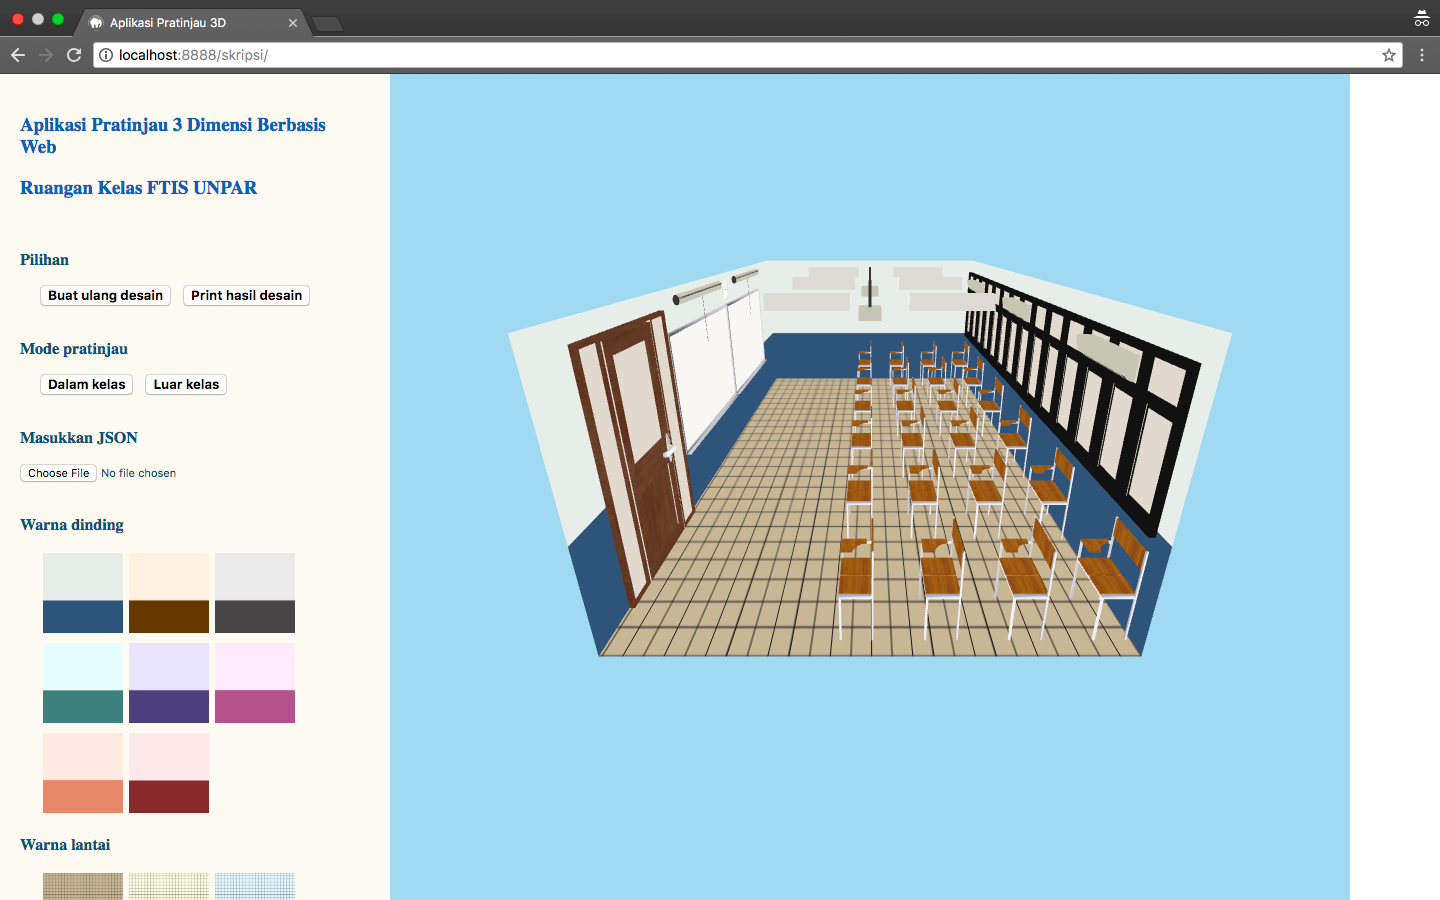
\includegraphics[scale=0.3]{ujitanpamejadosen}
	\caption{Hasil pengujian pemodelan ruangan kelas tanpa meja dosen.}
	\label{fig:ujitanpamejadosen}
\end{figure}
	
	\item {\bf Ruangan kelas dengan bentuk persegi.}
	
	Masukan untuk kasus uji ini merupakan sebuah berkas JSON yang dapat dilihat pada {\it listing} ~\ref{lst:ujikelaskotak}. Keluaran untuk kasus uji ini merupakan pemodelan ruangan kelas berbentuk perpegi dan penyesuaian properti untuk bentuk kelas persegi. Hasil pengujian dapat dilihat pada gambar ~\ref{fig:ujikelaskotak}.
\begin{lstlisting}[caption={Isi berkas JSON untuk pemodelan ruangan kelas berbentuk persegi.}, label={lst:ujikelaskotak},captionpos=b]
var constant = {
    "worldColor": 11131375,
    "control": {
        "minZoom": 15,
        "maxZoom": 42
    },
    "classProperties": [
    {
        "dx": 17.9,
        "dy": 4,
        "dz": 18.7,
        "distancex": -3,
        "distancez": -3.5,
        "repeatx": 6,
        "repeatz": 5,
        "rotation": 0,
        "texture": "models/texturekursimahasiswa.jpg",
        "model": "models/kursimahasiswa.json",
        "scale": 1
    },
    {
        "dx": -3.2,
        "dy": 4,
        "dz": 18.7,
        "distancex": -3,
        "distancez": -3.5,
        "repeatx": 6,
        "repeatz": 5,
        "rotation": 0,
        "texture": "models/texturekursimahasiswa.jpg",
        "model": "models/kursimahasiswa.json",
        "scale": 1
    },
    {
        "dx": -6,
        "dy": 10,
        "dz": -16.5,
        "distancex": 12.3,
        "distancez": 0,
        "repeatx": 2,
        "repeatz": 1,
        "rotation": 0,
        "texture": "models/texturepapantulis.jpg",
        "model": "models/papantulis.json",
        "scale": 3.5
    },
    {
        "dx": 17.5,
        "dy": 10.2,
        "dz": 21.7,
        "distancex": -3,
        "distancez": 0,
        "repeatx": 13,
        "repeatz": 1,
        "rotation": 3.14159,
        "texture": "models/texturejendela.jpg",
        "model": "models/jendela.json",
        "scale": 2
    },
    {
        "dx": 8,
        "dy": 4.7,
        "dz": -8,
        "distancex": 6,
        "distancez": 0,
        "repeatx": 2,
        "repeatz": 1,
        "rotation": 4.712385,
        "texture": "models/texturemejadosen.jpg",
        "model": "models/mejadosen.json",
        "scale": 2
    },
    {
        "dx": -8,
        "dy": 14.5,
        "dz": -19.6,
        "distancex": 13,
        "distancez": 0,
        "repeatx": 2,
        "repeatz": 1,
        "rotation": 0,
        "texture": "models/textureacproyektorlayar.jpg",
        "model": "models/layar.json",
        "scale": 1
    },
    {
        "dx": -4,
        "dy": 14,
        "dz": 0,
        "distancex": 13,
        "distancez": 0,
        "repeatx": 2,
        "repeatz": 1,
        "rotation": 3.14159,
        "texture": "models/textureacproyektorlayar.jpg",
        "model": "models/proyektor.json",
        "scale": 1
    },
    {
        "dx": -15,
        "dy": 13,
        "dz": 14.5,
        "distancex": 15,
        "distancez": 0,
        "repeatx": 3,
        "repeatz": 1,
        "rotation": 3.14159,
        "texture": "models/textureacproyektorlayar.jpg",
        "model": "models/ac.json",
        "scale": 1
    },
    {
        "dx": -13,
        "dy": 14.9,
        "dz": -5,
        "distancex": 10,
        "distancez": 10,
        "repeatx": 3,
        "repeatz": 2,
        "rotation": 0,
        "texture": "models/texturelampu.jpg",
        "model": "models/lampu.json",
        "scale": 1
    },
    {
        "dx": 2.7,
        "dy": 14,
        "dz": -15.2,
        "distancex": 0,
        "distancez": 0,
        "repeatx": 1,
        "repeatz": 1,
        "rotation": 0,
        "texture": "models/texturejamdinding.jpg",
        "model": "models/jamdinding.json",
        "scale": 1
    },
    {
        "dx": -13,
        "dy": 7.5,
        "dz": -19.1,
        "distancex": 0,
        "distancez": 0,
        "repeatx": 1,
        "repeatz": 1,
        "rotation": 0,
        "texture": "models/texturepintu.jpg",
        "model": "models/pintu.json",
        "scale": 2
    },
    {
        "dx": 10,
        "dy": 5.5,
        "dz": -12,
        "distancex": 0,
        "distancez": 0,
        "repeatx": 1,
        "repeatz": 1,
        "rotation": 0,
        "texture": "models/texturekursidosen.jpg",
        "model": "models/kursidosen.json",
        "scale": 1.5
    }
],
"room": {
    "texture": {
        "wall": [
            "img/texturedinding1.jpg",
            "img/texturedinding2.jpg",
            "img/texturedinding3.jpg",
            "img/texturedinding4.jpg",
            "img/texturedinding5.jpg",
            "img/texturedinding6.jpg",
            "img/texturedinding7.jpg",
            "img/texturedinding8.jpg"
        ],
        "floor": [
            "img/texturelantai1.jpg",
            "img/texturelantai2.jpg",
            "img/texturelantai3.jpg",
            "img/texturelantai4.jpg",
            "img/texturelantai5.jpg",
            "img/texturelantai6.jpg",
            "img/texturelantai7.jpg",
            "img/texturelantai8.jpg"
        ],
        "ceiling": "img/textureatap.jpg"
    },
    "size": {
        "length": 40,
        "width": 12,
        "height": 40
    }
},
"view": {
    "outside": {
        "cameraPosition": {
            "x": 0,
            "y": 10,
            "z": 40
        },
        "control": {
            "minZoom": 10,
            "maxZoom": 42
        },
        "target": {
            "x": 0,
            "y": 10,
            "z": 0
        }
    },
    "inside": {
        "cameraPosition": {
            "x": 0,
            "y": 10,
            "z": 0
        },
        "control": {
            "minZoom": 5,
            "maxZoom": 15
        },
        "target": {
            "x": 0,
            "y": 10,
            "z": 0
        }
    },
    "init": {
        "verticalField": 75,
        "nearPlane": 0.1,
        "farPlane": 100
    }
} 
}
\end{lstlisting}

\begin{figure}[H]
	\centering
	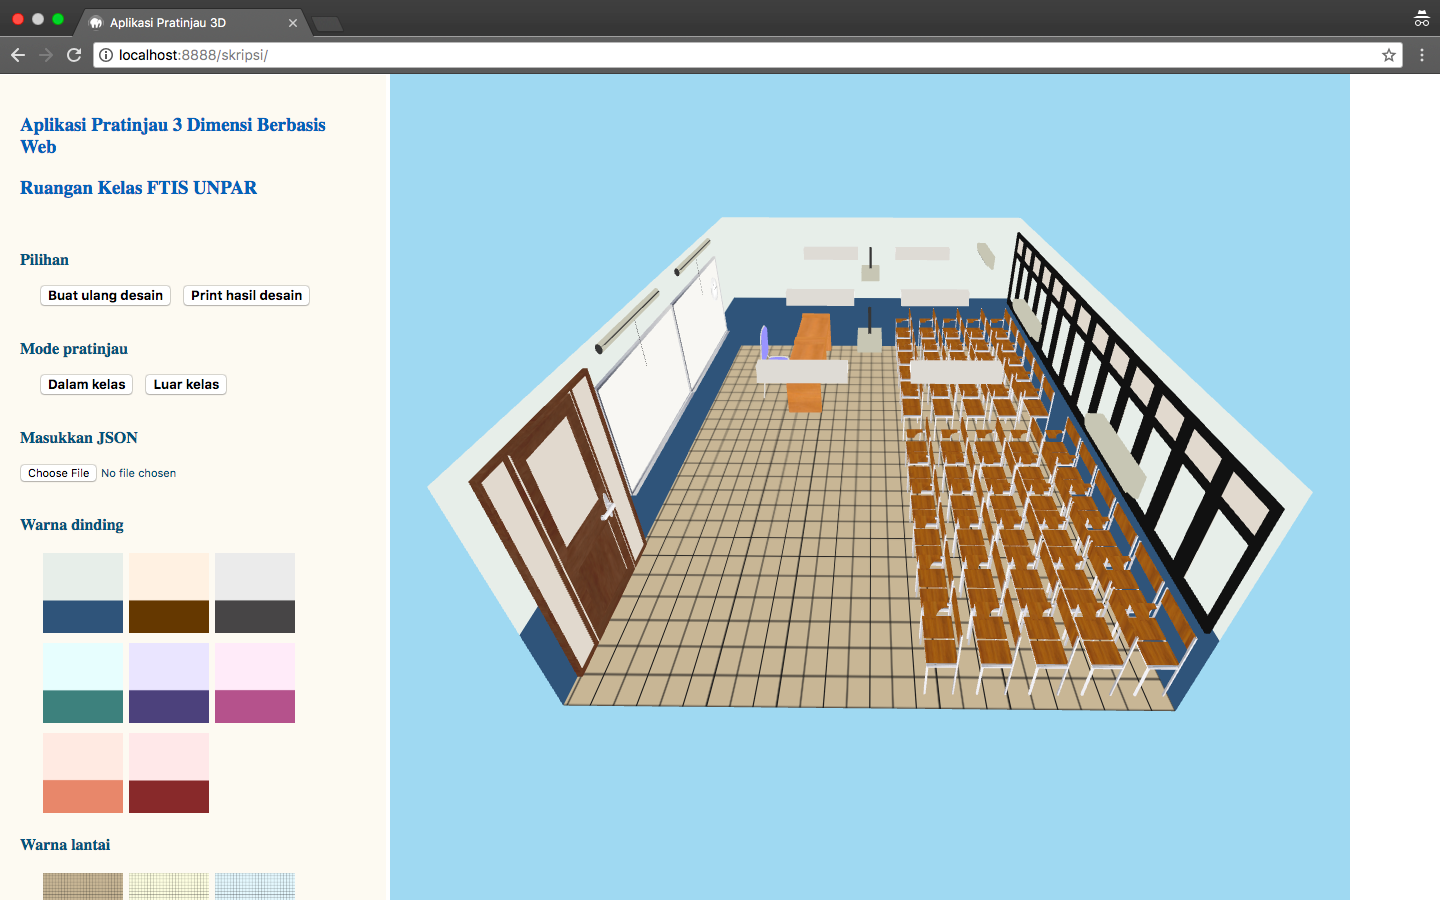
\includegraphics[scale=0.3]{ujikelaskotak}
	\caption{Hasil pengujian pemodelan ruangan kelas berbentuk persegi.}
	\label{fig:ujikelaskotak}
\end{figure}
	
	\item {\bf Ruangan kelas dengan bentuk memanjang.}
	
	Masukan untuk kasus uji ini merupakan sebuah berkas JSON yang dapat dilihat pada {\it listing} ~\ref{lst:ujikelaspanjang}. Keluaran untuk kasus uji ini merupakan pemodelan ruangan kelas berbentuk memanjang dan penyesuaian properti untuk bentuk kelas tersebut. Hasil pengujian dapat dilihat pada gambar ~\ref{fig:ujikelaspanjang}.
\begin{lstlisting}[caption={Isi berkas JSON untuk pemodelan ruangan kelas berbentuk memanjang.}, label={lst:ujikelaspanjang},captionpos=b]
{
    "worldColor": 11131375,
    "control": {
        "minZoom": 15,
        "maxZoom": 42
    },
    "classProperties": [
    {
        "dx": 7.2,
        "dy": 4,
        "dz": 23.7,
        "distancex": -3,
        "distancez": -3.5,
        "repeatx": 5,
        "repeatz": 8,
        "rotation": 0,
        "texture": "models/texturekursimahasiswa.jpg",
        "model": "models/kursimahasiswa.json",
        "scale": 1
    },
    {
        "dx": -1,
        "dy": 10,
        "dz": -21.5,
        "distancex": 12.3,
        "distancez": 0,
        "repeatx": 1,
        "repeatz": 1,
        "rotation": 0,
        "texture": "models/texturepapantulis.jpg",
        "model": "models/papantulis.json",
        "scale": 3.5
    },
    {
        "dx": 7,
        "dy": 10.2,
        "dz": 26.7,
        "distancex": -3,
        "distancez": 0,
        "repeatx": 6,
        "repeatz": 1,
        "rotation": 3.14159,
        "texture": "models/texturejendela.jpg",
        "model": "models/jendela.json",
        "scale": 2
    },
    {
        "dx": -8,
        "dy": 4.7,
        "dz": -12,
        "distancex": 6,
        "distancez": 0,
        "repeatx": 2,
        "repeatz": 1,
        "rotation": 4.712385,
        "texture": "models/texturemejadosen.jpg",
        "model": "models/mejadosen.json",
        "scale": 2
    },
    {
        "dx": -2,
        "dy": 14.5,
        "dz": -24.6,
        "distancex": 13,
        "distancez": 0,
        "repeatx": 1,
        "repeatz": 1,
        "rotation": 0,
        "texture": "models/textureacproyektorlayar.jpg",
        "model": "models/layar.json",
        "scale": 1
    },
    {
        "dx": 2,
        "dy": 14,
        "dz": -5,
        "distancex": 13,
        "distancez": 0,
        "repeatx": 1,
        "repeatz": 1,
        "rotation": 3.14159,
        "texture": "models/textureacproyektorlayar.jpg",
        "model": "models/proyektor.json",
        "scale": 1
    },
    {
        "dx": -7,
        "dy": 13,
        "dz": 24,
        "distancex": 10,
        "distancez": 0,
        "repeatx": 2,
        "repeatz": 1,
        "rotation": 3.14159,
        "texture": "models/textureacproyektorlayar.jpg",
        "model": "models/ac.json",
        "scale": 1
    },
    {
        "dx": -8,
        "dy": 14.9,
        "dz": -5,
        "distancex": 10,
        "distancez": 10,
        "repeatx": 2,
        "repeatz": 3,
        "rotation": 0,
        "texture": "models/texturelampu.jpg",
        "model": "models/lampu.json",
        "scale": 1
    },
    {
        "dx": 9,
        "dy": 7.5,
        "dz": -17.1,
        "distancex": 0,
        "distancez": 0,
        "repeatx": 1,
        "repeatz": 1,
        "rotation": 4.712385,
        "texture": "models/texturepintu.jpg",
        "model": "models/pintu.json",
        "scale": 2
    },
    {
        "dx": -5,
        "dy": 5.5,
        "dz": -16,
        "distancex": 0,
        "distancez": 0,
        "repeatx": 1,
        "repeatz": 1,
        "rotation": 0,
        "texture": "models/texturekursidosen.jpg",
        "model": "models/kursidosen.json",
        "scale": 1.5
    }
],
"room": {
    "texture": {
        "wall": [
            "img/texturedinding1.jpg",
            "img/texturedinding2.jpg",
            "img/texturedinding3.jpg",
            "img/texturedinding4.jpg",
            "img/texturedinding5.jpg",
            "img/texturedinding6.jpg",
            "img/texturedinding7.jpg",
            "img/texturedinding8.jpg"
        ],
        "floor": [
            "img/texturelantai1.jpg",
            "img/texturelantai2.jpg",
            "img/texturelantai3.jpg",
            "img/texturelantai4.jpg",
            "img/texturelantai5.jpg",
            "img/texturelantai6.jpg",
            "img/texturelantai7.jpg",
            "img/texturelantai8.jpg"
        ],
        "ceiling": "img/textureatap.jpg"
    },
    "size": {
        "length": 20,
        "width": 12,
        "height": 50
    }
},
"view": {
    "outside": {
        "cameraPosition": {
            "x": 0,
            "y": 10,
            "z": 40
        },
        "control": {
            "minZoom": 10,
            "maxZoom": 42
        },
        "target": {
            "x": 0,
            "y": 10,
            "z": 0
        }
    },
    "inside": {
        "cameraPosition": {
            "x": 0,
            "y": 10,
            "z": 0
        },
        "control": {
            "minZoom": 5,
            "maxZoom": 15
        },
        "target": {
            "x": 0,
            "y": 10,
            "z": 0
        }
    },
    "init": {
        "verticalField": 75,
        "nearPlane": 0.1,
        "farPlane": 100
    }
} 
}
\end{lstlisting}

\begin{figure}[H]
	\centering
	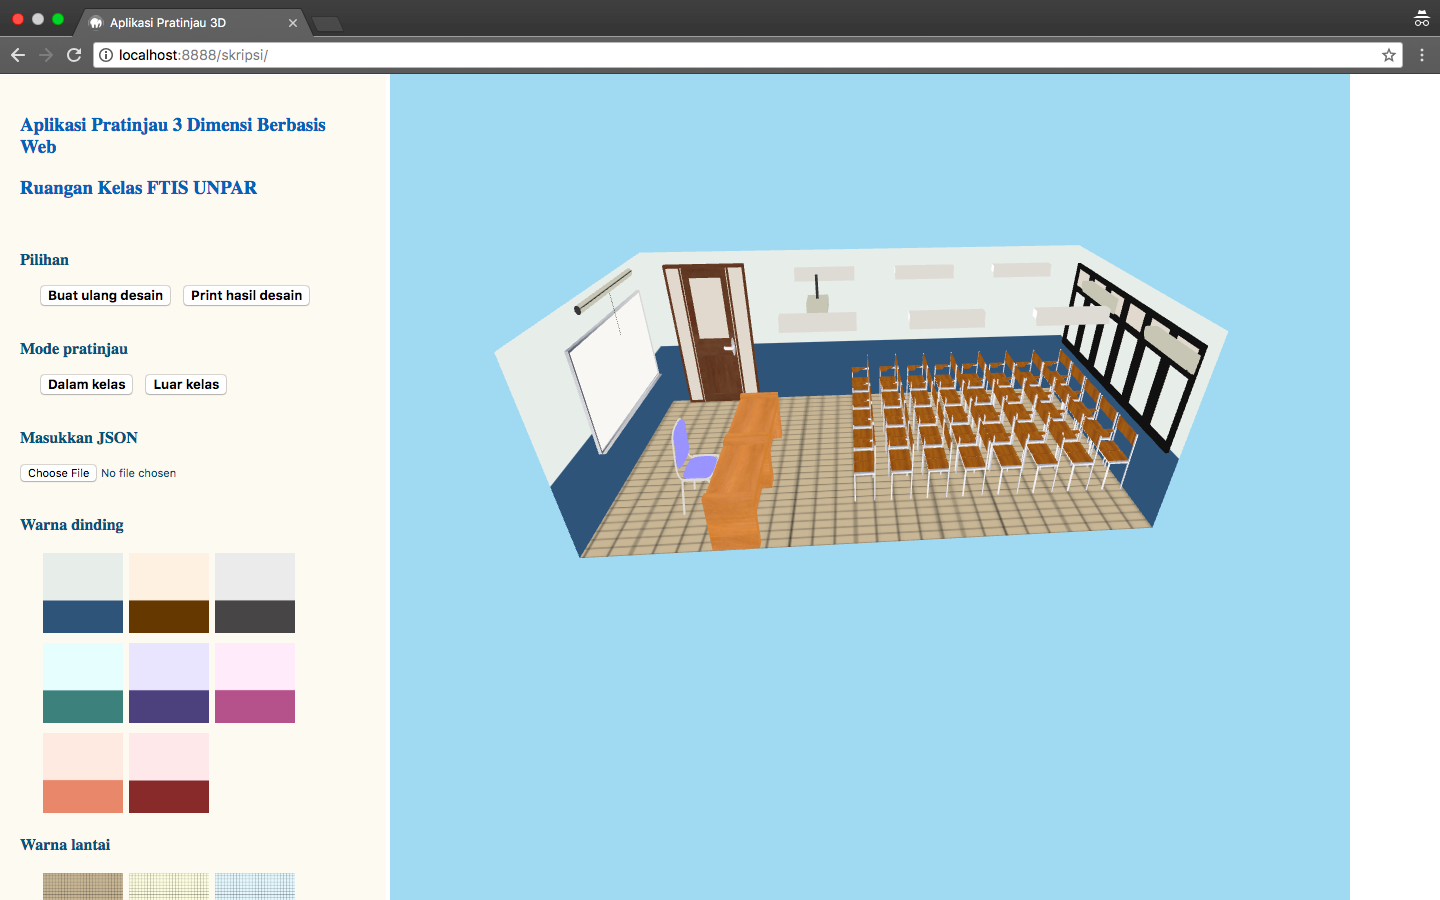
\includegraphics[scale=0.3]{ujikelaspanjang}
	\caption{Hasil pengujian pemodelan ruangan kelas memanjang.}
	\label{fig:ujikelaspanjang}
\end{figure}
	
	\item {\bf Dunia di luar ruangan kelas berwarna hitam.}
	
	Masukan untuk kasus uji ini merupakan sebuah berkas JSON yang dapat dilihat pada {\it listing} ~\ref{lst:ujiduniahitam}. Keluaran untuk kasus uji ini merupakan pemodelan ruangan kelas dengan dunia di luar ruangan berwarna hitam. Hasil pengujian dapat dilihat pada gambar ~\ref{fig:ujiduniahitam}.
\begin{lstlisting}[caption={Isi berkas JSON untuk pemodelan ruangan kelas dengan luar ruangan berwarna hitam.}, label={lst:ujiduniahitam},captionpos=b]
{
    "worldColor": 00000000,
    "control": {
        "minZoom": 15,
        "maxZoom": 42
    },
    "classProperties": [
        {
            "dx": 19.5,
            "dy": 4,
            "dz": 14.2,
            "distancex": -3,
            "distancez": -3.5,
            "repeatx": 6,
            "repeatz": 5,
            "rotation": 0,
            "texture": "models/texturekursimahasiswa.jpg",
            "model": "models/kursimahasiswa.json",
            "scale": 1
        },
        {
            "dx": -4,
            "dy": 4,
            "dz": 14.2,
            "distancex": -3,
            "distancez": -3.5,
            "repeatx": 6,
            "repeatz": 5,
            "rotation": 0,
            "texture": "models/texturekursimahasiswa.jpg",
            "model": "models/kursimahasiswa.json",
            "scale": 1
        },
        {
            "dx": -6,
            "dy": 10,
            "dz": -12,
            "distancex": 12.3,
            "distancez": 0,
            "repeatx": 2,
            "repeatz": 1,
            "rotation": 0,
            "texture": "models/texturepapantulis.jpg",
            "model": "models/papantulis.json",
            "scale": 3.5
        },
        {
            "dx": 19.5,
            "dy": 10.2,
            "dz": 17.1,
            "distancex": -3,
            "distancez": 0,
            "repeatx": 14,
            "repeatz": 1,
            "rotation": 3.14159,
            "texture": "models/texturejendela.jpg",
            "model": "models/jendela.json",
            "scale": 2
        },
        {
            "dx": 8,
            "dy": 4.7,
            "dz": -8,
            "distancex": 6,
            "distancez": 0,
            "repeatx": 2,
            "repeatz": 1,
            "rotation": 4.712385,
            "texture": "models/texturemejadosen.jpg",
            "model": "models/mejadosen.json",
            "scale": 2
        },
        {
            "dx": -8,
            "dy": 14.5,
            "dz": -14.9,
            "distancex": 13,
            "distancez": 0,
            "repeatx": 2,
            "repeatz": 1,
            "rotation": 0,
            "texture": "models/textureacproyektorlayar.jpg",
            "model": "models/layar.json",
            "scale": 1
        },
        {
            "dx": -4,
            "dy": 14,
            "dz": 0,
            "distancex": 13,
            "distancez": 0,
            "repeatx": 2,
            "repeatz": 1,
            "rotation": 3.14159,
            "texture": "models/textureacproyektorlayar.jpg",
            "model": "models/proyektor.json",
            "scale": 1
        },
        {
            "dx": -15,
            "dy": 13,
            "dz": 14.5,
            "distancex": 15,
            "distancez": 0,
            "repeatx": 3,
            "repeatz": 1,
            "rotation": 3.14159,
            "texture": "models/textureacproyektorlayar.jpg",
            "model": "models/ac.json",
            "scale": 1
        },
        {
            "dx": -13,
            "dy": 14.9,
            "dz": -5,
            "distancex": 10,
            "distancez": 10,
            "repeatx": 3,
            "repeatz": 2,
            "rotation": 0,
            "texture": "models/texturelampu.jpg",
            "model": "models/lampu.json",
            "scale": 1
        },
        {
            "dx": 2.7,
            "dy": 14,
            "dz": -15.2,
            "distancex": 0,
            "distancez": 0,
            "repeatx": 1,
            "repeatz": 1,
            "rotation": 0,
            "texture": "models/texturejamdinding.jpg",
            "model": "models/jamdinding.json",
            "scale": 1
        },
        {
            "dx": -13,
            "dy": 7.5,
            "dz": -14.6,
            "distancex": 0,
            "distancez": 0,
            "repeatx": 1,
            "repeatz": 1,
            "rotation": 0,
            "texture": "models/texturepintu.jpg",
            "model": "models/pintu.json",
            "scale": 2
        },
        {
            "dx": 10,
            "dy": 5.5,
            "dz": -12,
            "distancex": 0,
            "distancez": 0,
            "repeatx": 1,
            "repeatz": 1,
            "rotation": 0,
            "texture": "models/texturekursidosen.jpg",
            "model": "models/kursidosen.json",
            "scale": 1.5
        }
    ],
    "room": {
        "texture": {
            "wall": [
                "img/texturedinding1.jpg",
                "img/texturedinding2.jpg",
                "img/texturedinding3.jpg",
                "img/texturedinding4.jpg",
                "img/texturedinding5.jpg",
                "img/texturedinding6.jpg",
                "img/texturedinding7.jpg",
                "img/texturedinding8.jpg"
            ],
            "floor": [
                "img/texturelantai1.jpg",
                "img/texturelantai2.jpg",
                "img/texturelantai3.jpg",
                "img/texturelantai4.jpg",
                "img/texturelantai5.jpg",
                "img/texturelantai6.jpg",
                "img/texturelantai7.jpg",
                "img/texturelantai8.jpg"
            ],
            "ceiling": "img/textureatap.jpg"
        },
        "size": {
            "length": 43,
            "width": 12,
            "height": 31
        }
    },
    "view": {
        "outside": {
            "cameraPosition": {
                "x": 0,
                "y": 10,
                "z": 40
            },
            "control": {
                "minZoom": 10,
                "maxZoom": 42
            },
            "target": {
                "x": 0,
                "y": 10,
                "z": 0
            }
        },
        "inside": {
            "cameraPosition": {
                "x": 0,
                "y": 10,
                "z": 0
            },
            "control": {
                "minZoom": 5,
                "maxZoom": 15
            },
            "target": {
                "x": 0,
                "y": 10,
                "z": 0
            }
        },
        "init": {
            "verticalField": 75,
            "nearPlane": 0.1,
            "farPlane": 100
        }
    } 
}
\end{lstlisting}

\begin{figure}[H]
	\centering
	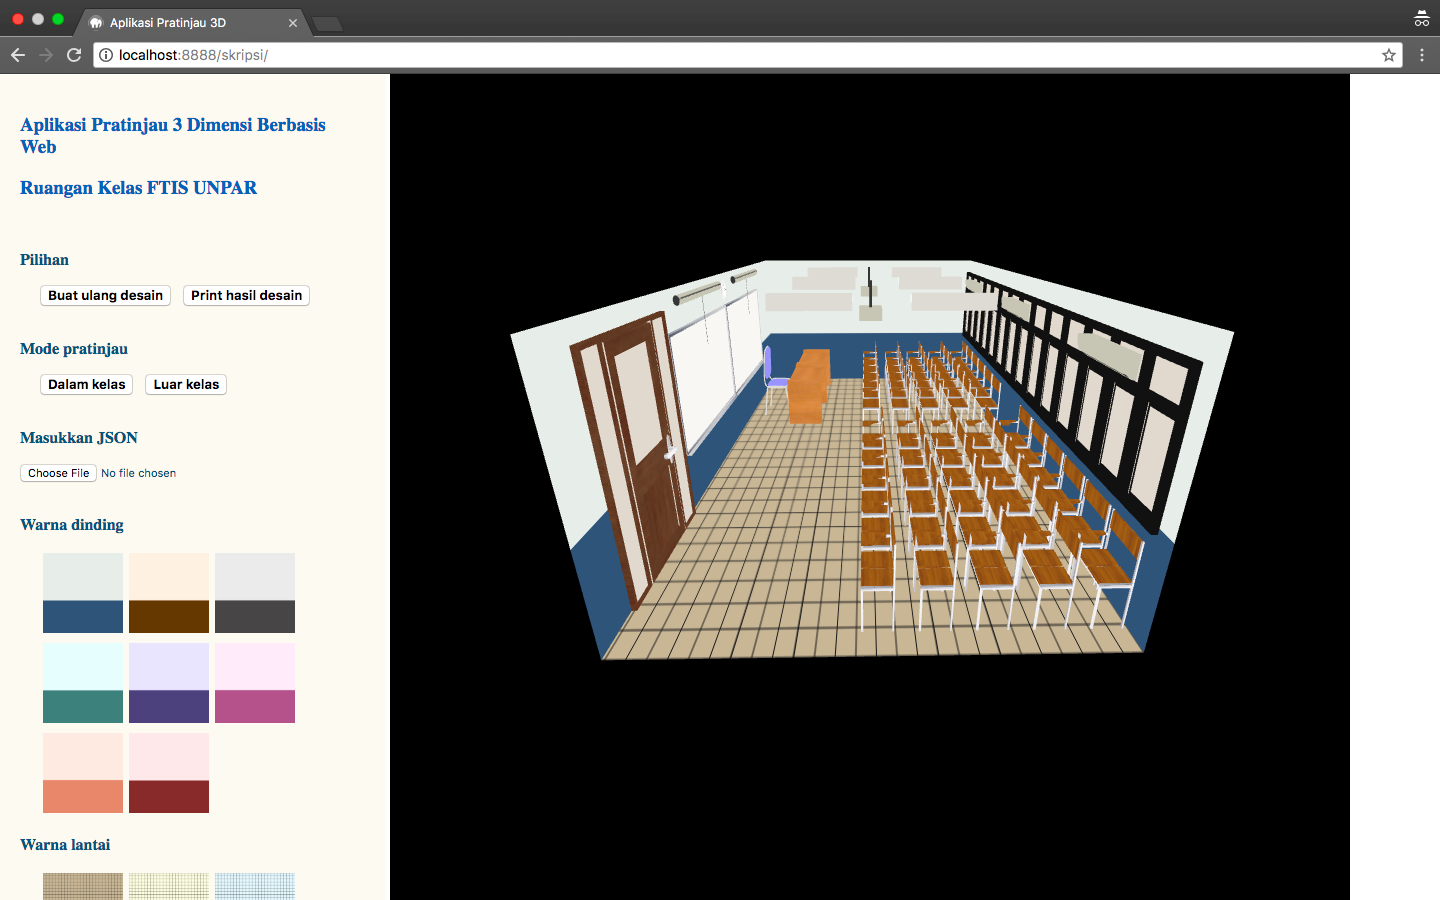
\includegraphics[scale=0.3]{ujiduniahitam}
	\caption{Hasil pengujian pemodelan ruangan kelas dengan luar ruangan berwarna hitam.}
	\label{fig:ujiduniahitam}
\end{figure}
	
\end{itemize}

\subsection{Mengganti Pilihan Tekstur Warna Dinding untuk Ruangan Kelas}
\label{sec:pilihanteksturdinding}

	Masukan untuk kasus uji ini merupakan sebuah berkas JSON yang dapat dilihat pada {\it listing} ~\ref{lst:ujipilihandinding}. Masukan untuk uji kasus ini berfokus pada objek {\it room} yang ada pada berkas JSON ini. Keluaran untuk kasus uji ini merupakan pilihan tekstur dinding baru untuk digunakan pada pemodelan ruangan kelas. Hasil pengujian dapat dilihat pada gambar ~\ref{fig:ujipilihandinding}.
\begin{lstlisting}[caption={Isi berkas JSON untuk mengganti pilihan tekstur dinding.}, label={lst:ujipilihandinding},captionpos=b]
{
    "worldColor": 11131375,
    "control": {
        "minZoom": 15,
        "maxZoom": 42
    },
    "classProperties": [
        {
            "dx": 19.5,
            "dy": 4,
            "dz": 14.2,
            "distancex": -3,
            "distancez": -3.5,
            "repeatx": 6,
            "repeatz": 5,
            "rotation": 0,
            "texture": "models/texturekursimahasiswa.jpg",
            "model": "models/kursimahasiswa.json",
            "scale": 1
        },
        {
            "dx": -4,
            "dy": 4,
            "dz": 14.2,
            "distancex": -3,
            "distancez": -3.5,
            "repeatx": 6,
            "repeatz": 5,
            "rotation": 0,
            "texture": "models/texturekursimahasiswa.jpg",
            "model": "models/kursimahasiswa.json",
            "scale": 1
        },
        {
            "dx": -6,
            "dy": 10,
            "dz": -12,
            "distancex": 12.3,
            "distancez": 0,
            "repeatx": 2,
            "repeatz": 1,
            "rotation": 0,
            "texture": "models/texturepapantulis.jpg",
            "model": "models/papantulis.json",
            "scale": 3.5
        },
        {
            "dx": 19.5,
            "dy": 10.2,
            "dz": 17.1,
            "distancex": -3,
            "distancez": 0,
            "repeatx": 14,
            "repeatz": 1,
            "rotation": 3.14159,
            "texture": "models/texturejendela.jpg",
            "model": "models/jendela.json",
            "scale": 2
        },
        {
            "dx": 8,
            "dy": 4.7,
            "dz": -8,
            "distancex": 6,
            "distancez": 0,
            "repeatx": 2,
            "repeatz": 1,
            "rotation": 4.712385,
            "texture": "models/texturemejadosen.jpg",
            "model": "models/mejadosen.json",
            "scale": 2
        },
        {
            "dx": -8,
            "dy": 14.5,
            "dz": -14.9,
            "distancex": 13,
            "distancez": 0,
            "repeatx": 2,
            "repeatz": 1,
            "rotation": 0,
            "texture": "models/textureacproyektorlayar.jpg",
            "model": "models/layar.json",
            "scale": 1
        },
        {
            "dx": -4,
            "dy": 14,
            "dz": 0,
            "distancex": 13,
            "distancez": 0,
            "repeatx": 2,
            "repeatz": 1,
            "rotation": 3.14159,
            "texture": "models/textureacproyektorlayar.jpg",
            "model": "models/proyektor.json",
            "scale": 1
        },
        {
            "dx": -15,
            "dy": 13,
            "dz": 14.5,
            "distancex": 15,
            "distancez": 0,
            "repeatx": 3,
            "repeatz": 1,
            "rotation": 3.14159,
            "texture": "models/textureacproyektorlayar.jpg",
            "model": "models/ac.json",
            "scale": 1
        },
        {
            "dx": -13,
            "dy": 14.9,
            "dz": -5,
            "distancex": 10,
            "distancez": 10,
            "repeatx": 3,
            "repeatz": 2,
            "rotation": 0,
            "texture": "models/texturelampu.jpg",
            "model": "models/lampu.json",
            "scale": 1
        },
        {
            "dx": 2.7,
            "dy": 14,
            "dz": -15.2,
            "distancex": 0,
            "distancez": 0,
            "repeatx": 1,
            "repeatz": 1,
            "rotation": 0,
            "texture": "models/texturejamdinding.jpg",
            "model": "models/jamdinding.json",
            "scale": 1
        },
        {
            "dx": -13,
            "dy": 7.5,
            "dz": -14.6,
            "distancex": 0,
            "distancez": 0,
            "repeatx": 1,
            "repeatz": 1,
            "rotation": 0,
            "texture": "models/texturepintu.jpg",
            "model": "models/pintu.json",
            "scale": 2
        },
        {
            "dx": 10,
            "dy": 5.5,
            "dz": -12,
            "distancex": 0,
            "distancez": 0,
            "repeatx": 1,
            "repeatz": 1,
            "rotation": 0,
            "texture": "models/texturekursidosen.jpg",
            "model": "models/kursidosen.json",
            "scale": 1.5
        }
    ],
    "room": {
        "texture": {
            "wall": [
                "img/teksturdindingbaru1.jpg",
                "img/teksturdindingbaru2.jpg",
                "img/teksturdindingbaru3.jpeg",
                "img/teksturdindingbaru4.jpg"
            ],
            "floor": [
                "img/texturelantai1.jpg",
                "img/texturelantai2.jpg",
                "img/texturelantai3.jpg",
                "img/texturelantai4.jpg",
                "img/texturelantai5.jpg",
                "img/texturelantai6.jpg",
                "img/texturelantai7.jpg",
                "img/texturelantai8.jpg"
            ],
            "ceiling": "img/textureatap.jpg"
        },
        "size": {
            "length": 43,
            "width": 12,
            "height": 31
        }
    },
    "view": {
        "outside": {
            "cameraPosition": {
                "x": 0,
                "y": 10,
                "z": 40
            },
            "control": {
                "minZoom": 10,
                "maxZoom": 42
            },
            "target": {
                "x": 0,
                "y": 10,
                "z": 0
            }
        },
        "inside": {
            "cameraPosition": {
                "x": 0,
                "y": 10,
                "z": 0
            },
            "control": {
                "minZoom": 5,
                "maxZoom": 15
            },
            "target": {
                "x": 0,
                "y": 10,
                "z": 0
            }
        },
        "init": {
            "verticalField": 75,
            "nearPlane": 0.1,
            "farPlane": 100
        }
    } 
}
\end{lstlisting}

\begin{figure}[H]
	\centering
	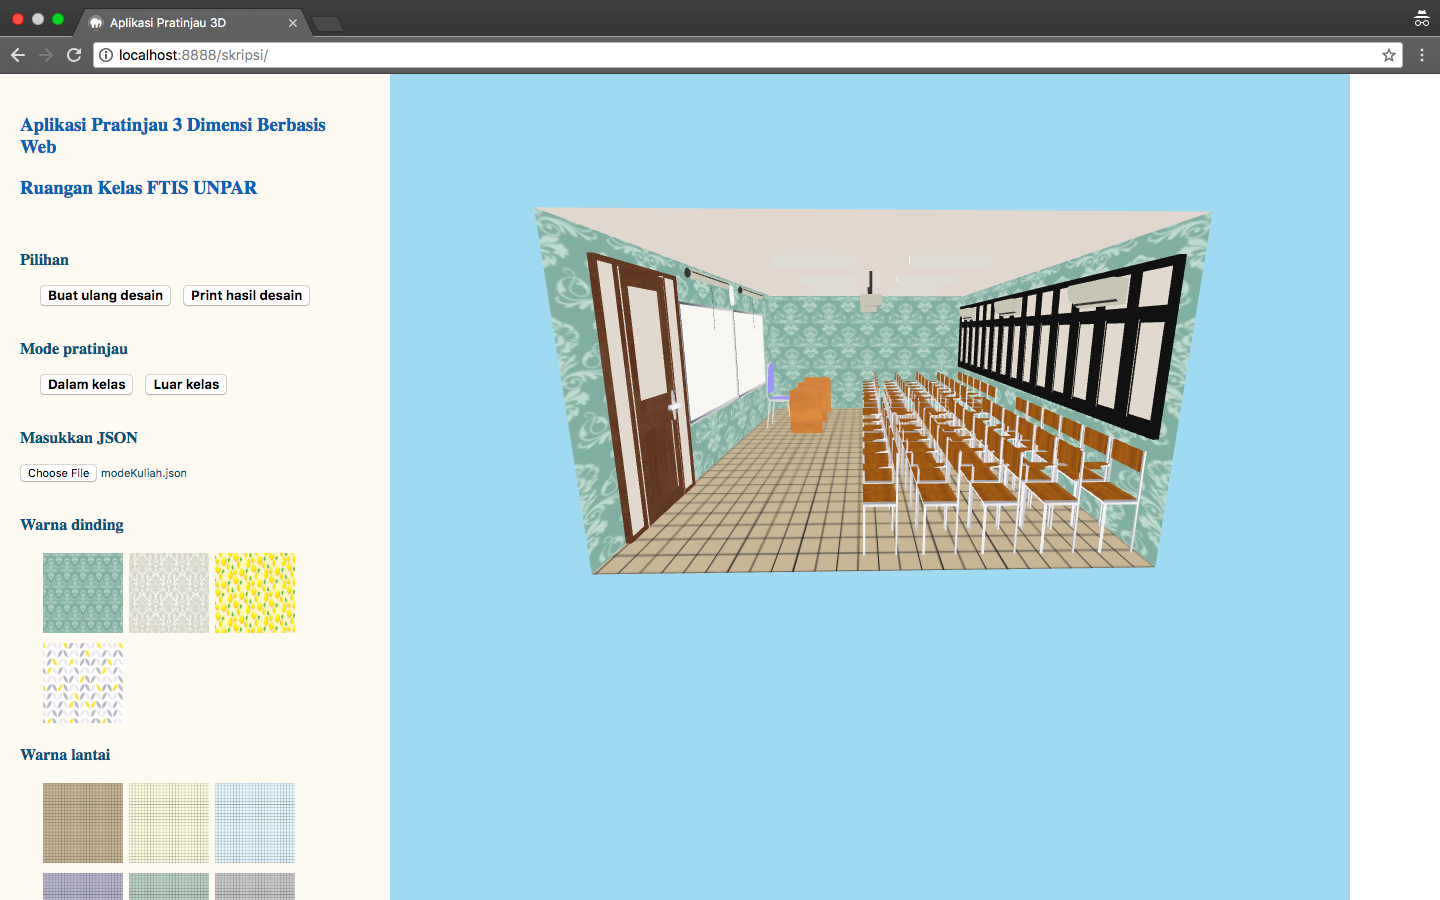
\includegraphics[scale=0.3]{ujipilihandinding}
	\caption{Hasil pengujian mengganti pilihan tekstur dinding.}
	\label{fig:ujipilihandinding}
\end{figure}

\subsection{Mengganti Pilihan Tekstur Warna Lantai untuk Ruangan Kelas}
\label{sec:pilihanteksturlantai}

Masukan untuk kasus uji ini merupakan sebuah berkas JSON yang dapat dilihat pada {\it listing} ~\ref{lst:ujipilihanlantai}. Masukan untuk uji kasus ini berfokus pada objek {\it room} yang ada pada berkas JSON ini. Keluaran untuk kasus uji ini merupakan pilihan tekstur lantai baru untuk digunakan pada pemodelan ruangan kelas. Hasil pengujian dapat dilihat pada gambar ~\ref{fig:ujipilihanlantai}.
\begin{lstlisting}[caption={Isi berkas JSON untuk mengganti pilihan tekstur lantai.}, label={lst:ujipilihanlantai},captionpos=b]
{
    "worldColor": 11131375,
    "control": {
        "minZoom": 15,
        "maxZoom": 42
    },
    "classProperties": [
        {
            "dx": 19.5,
            "dy": 4,
            "dz": 14.2,
            "distancex": -3,
            "distancez": -3.5,
            "repeatx": 6,
            "repeatz": 5,
            "rotation": 0,
            "texture": "models/texturekursimahasiswa.jpg",
            "model": "models/kursimahasiswa.json",
            "scale": 1
        },
        {
            "dx": -4,
            "dy": 4,
            "dz": 14.2,
            "distancex": -3,
            "distancez": -3.5,
            "repeatx": 6,
            "repeatz": 5,
            "rotation": 0,
            "texture": "models/texturekursimahasiswa.jpg",
            "model": "models/kursimahasiswa.json",
            "scale": 1
        },
        {
            "dx": -6,
            "dy": 10,
            "dz": -12,
            "distancex": 12.3,
            "distancez": 0,
            "repeatx": 2,
            "repeatz": 1,
            "rotation": 0,
            "texture": "models/texturepapantulis.jpg",
            "model": "models/papantulis.json",
            "scale": 3.5
        },
        {
            "dx": 19.5,
            "dy": 10.2,
            "dz": 17.1,
            "distancex": -3,
            "distancez": 0,
            "repeatx": 14,
            "repeatz": 1,
            "rotation": 3.14159,
            "texture": "models/texturejendela.jpg",
            "model": "models/jendela.json",
            "scale": 2
        },
        {
            "dx": 8,
            "dy": 4.7,
            "dz": -8,
            "distancex": 6,
            "distancez": 0,
            "repeatx": 2,
            "repeatz": 1,
            "rotation": 4.712385,
            "texture": "models/texturemejadosen.jpg",
            "model": "models/mejadosen.json",
            "scale": 2
        },
        {
            "dx": -8,
            "dy": 14.5,
            "dz": -14.9,
            "distancex": 13,
            "distancez": 0,
            "repeatx": 2,
            "repeatz": 1,
            "rotation": 0,
            "texture": "models/textureacproyektorlayar.jpg",
            "model": "models/layar.json",
            "scale": 1
        },
        {
            "dx": -4,
            "dy": 14,
            "dz": 0,
            "distancex": 13,
            "distancez": 0,
            "repeatx": 2,
            "repeatz": 1,
            "rotation": 3.14159,
            "texture": "models/textureacproyektorlayar.jpg",
            "model": "models/proyektor.json",
            "scale": 1
        },
        {
            "dx": -15,
            "dy": 13,
            "dz": 14.5,
            "distancex": 15,
            "distancez": 0,
            "repeatx": 3,
            "repeatz": 1,
            "rotation": 3.14159,
            "texture": "models/textureacproyektorlayar.jpg",
            "model": "models/ac.json",
            "scale": 1
        },
        {
            "dx": -13,
            "dy": 14.9,
            "dz": -5,
            "distancex": 10,
            "distancez": 10,
            "repeatx": 3,
            "repeatz": 2,
            "rotation": 0,
            "texture": "models/texturelampu.jpg",
            "model": "models/lampu.json",
            "scale": 1
        },
        {
            "dx": 2.7,
            "dy": 14,
            "dz": -15.2,
            "distancex": 0,
            "distancez": 0,
            "repeatx": 1,
            "repeatz": 1,
            "rotation": 0,
            "texture": "models/texturejamdinding.jpg",
            "model": "models/jamdinding.json",
            "scale": 1
        },
        {
            "dx": -13,
            "dy": 7.5,
            "dz": -14.6,
            "distancex": 0,
            "distancez": 0,
            "repeatx": 1,
            "repeatz": 1,
            "rotation": 0,
            "texture": "models/texturepintu.jpg",
            "model": "models/pintu.json",
            "scale": 2
        },
        {
            "dx": 10,
            "dy": 5.5,
            "dz": -12,
            "distancex": 0,
            "distancez": 0,
            "repeatx": 1,
            "repeatz": 1,
            "rotation": 0,
            "texture": "models/texturekursidosen.jpg",
            "model": "models/kursidosen.json",
            "scale": 1.5
        }
    ],
    "room": {
        "texture": {
            "wall": [
                "img/texturedinding1.jpg",
                "img/texturedinding2.jpg",
                "img/texturedinding3.jpg",
                "img/texturedinding4.jpg",
                "img/texturedinding5.jpg",
                "img/texturedinding6.jpg",
                "img/texturedinding7.jpg",
                "img/texturedinding8.jpg"
            ],
            "floor": [
                "img/teksturlantaibaru1.jpg",
                "img/teksturlantaibaru2.jpg",
                "img/teksturlantaibaru3.jpg",
                "img/teksturlantaibaru4.jpeg"
            ],
            "ceiling": "img/textureatap.jpg"
        },
        "size": {
            "length": 43,
            "width": 12,
            "height": 31
        }
    },
    "view": {
        "outside": {
            "cameraPosition": {
                "x": 0,
                "y": 10,
                "z": 40
            },
            "control": {
                "minZoom": 10,
                "maxZoom": 42
            },
            "target": {
                "x": 0,
                "y": 10,
                "z": 0
            }
        },
        "inside": {
            "cameraPosition": {
                "x": 0,
                "y": 10,
                "z": 0
            },
            "control": {
                "minZoom": 5,
                "maxZoom": 15
            },
            "target": {
                "x": 0,
                "y": 10,
                "z": 0
            }
        },
        "init": {
            "verticalField": 75,
            "nearPlane": 0.1,
            "farPlane": 100
        }
    } 
}
\end{lstlisting}

\begin{figure}[H]
	\centering
	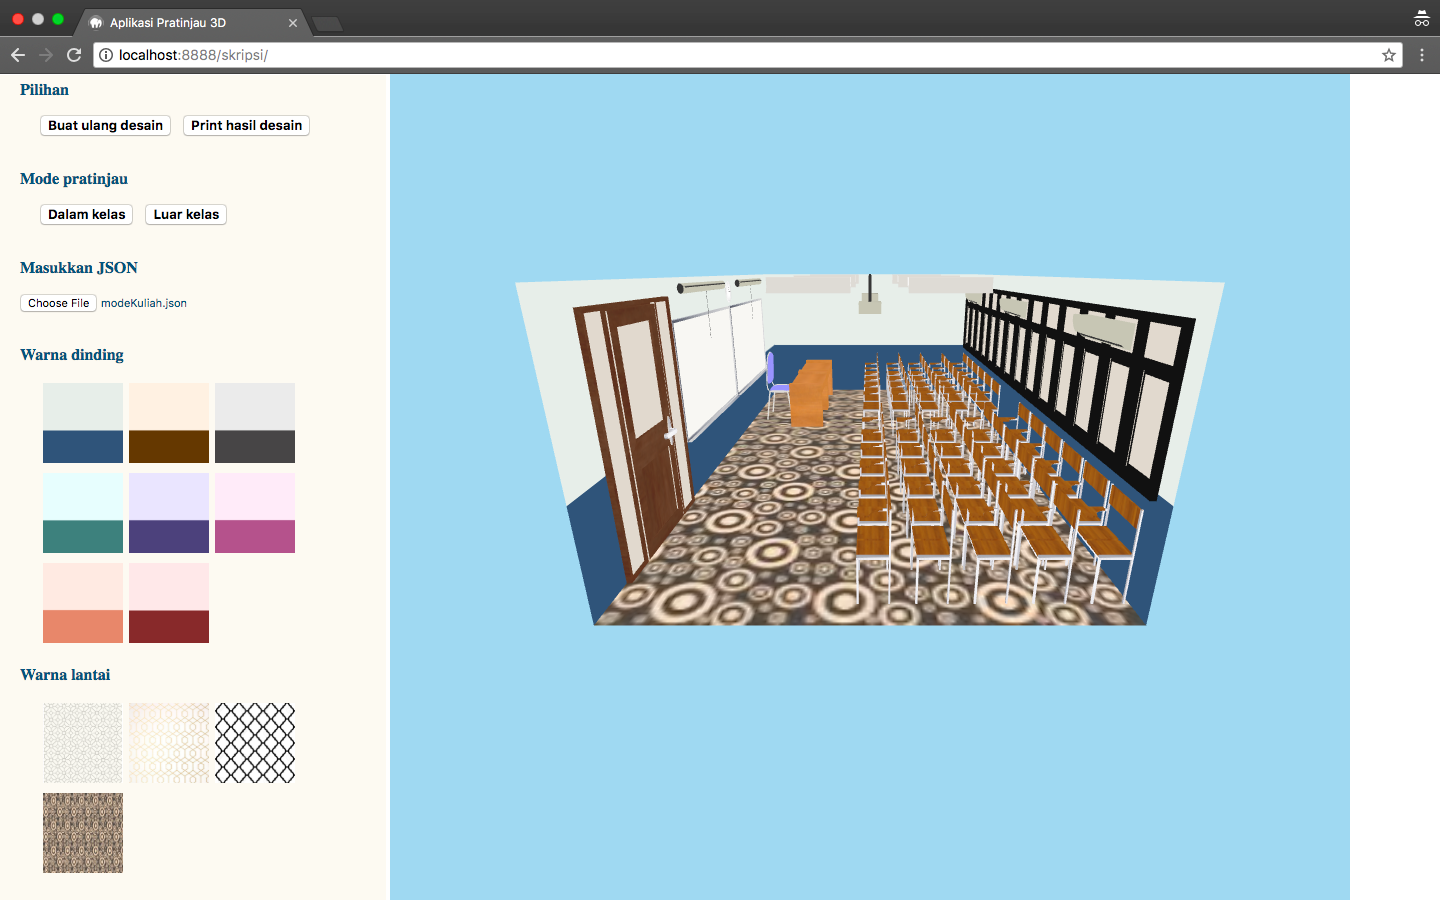
\includegraphics[scale=0.3]{ujipilihanlantai}
	\caption{Hasil pengujian mengganti pilihan tekstur lantai.}
	\label{fig:ujipilihanlantai}
\end{figure}

\subsection{Hasil Cetakan Berhasil Mengambil Gambar Ruangan Kelas}
Masukan untuk kasus uji ini merupakan pilihan pengguna untuk mencetak hasil pratinjau pemodelan ruangan kelas. Keluaran untuk kasus uji ini merupakan pratinjau hasil cetak pemodelan ruangan kelas tanpa menu pilihan pada web. Hasil pengujian dapat dilihat pada gambar ~\ref{fig:ujicetak}.
\begin{figure}[H]
	\centering
	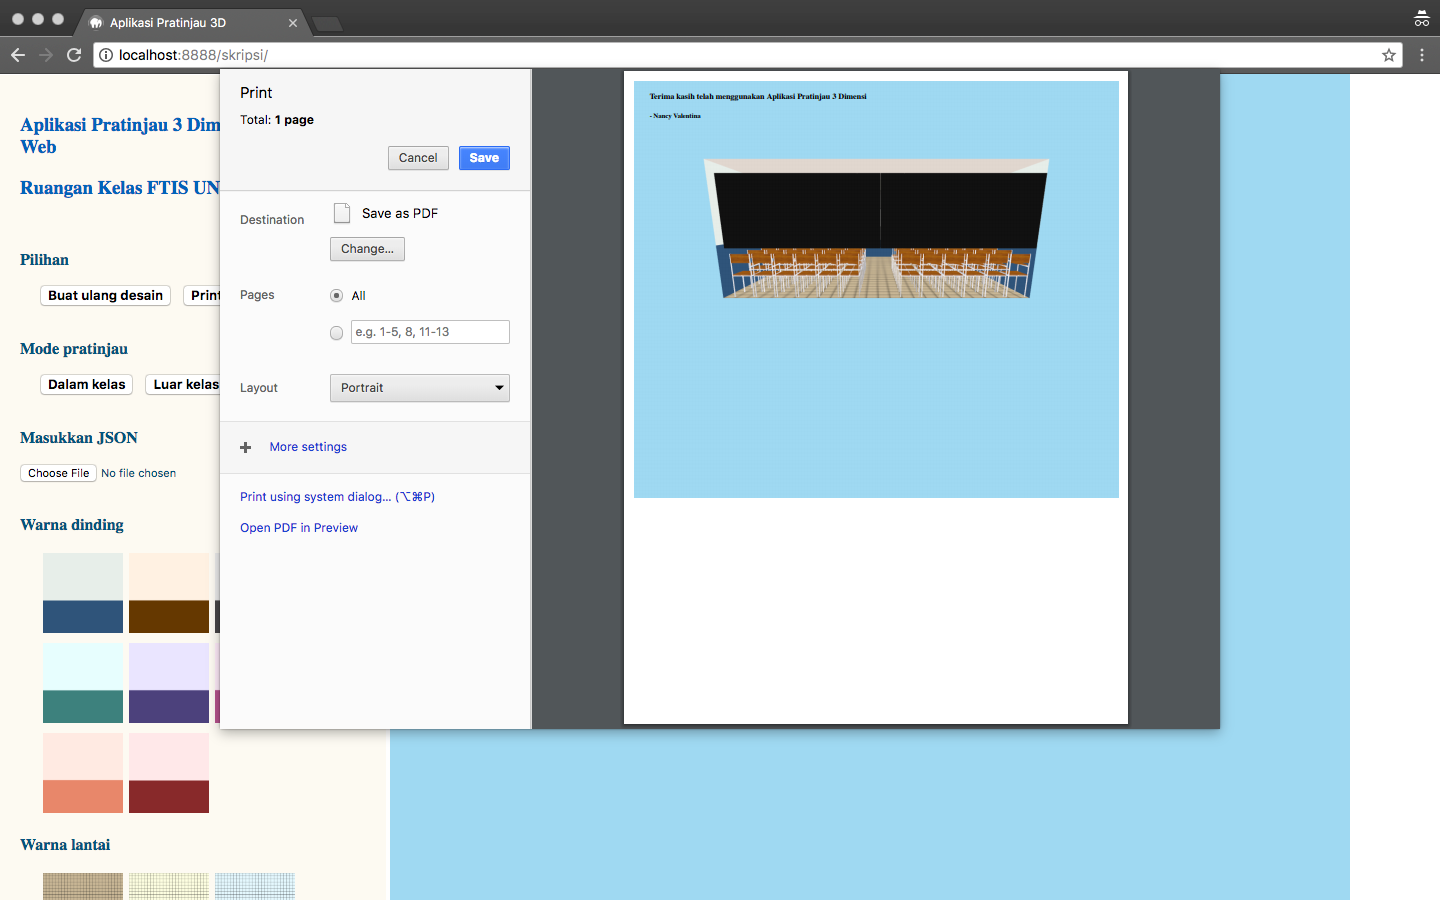
\includegraphics[scale=0.3]{ujicetak}
	\caption{Hasil pengujian pratinjau hasil cetak pemodelan ruangan kelas.}
	\label{fig:ujicetak}
\end{figure}
\label{sec:hasilcetakan}

















